\documentclass[12pt]{amsart}
\usepackage{amsmath, graphicx, color, slashed}
\addtolength{\textwidth}{4 truecm}
\addtolength{\textheight}{1 truecm}
\setlength{\voffset}{-.6 truecm}
\setlength{\hoffset}{-2.3 truecm}

\usepackage[all]{xy}
\xyoption{import}
\usepackage{amsthm}
\usepackage{mathrsfs}
%\usepackage[scaled=0.92]{helvet}	
%\renewcommand{\rmdefault}{ptm}	
%\usepackage[mtpcal,subscriptcorrection,nofontinfo]{mtpro2}
%\usepackage{lucimatx}
\usepackage[shortalphabetic]{amsrefs}


\newcommand{\spec}{\operatorname{spec}}
\DeclareMathOperator{\paulivec}{\boldsymbol{\sigma}}
\newcommand{\supp}{\operatorname{supp}}
\newcommand{\tr}{\operatorname{tr}}
\newcommand{\Tr}{\operatorname{Tr}}
\newcommand{\op}[1]{\widehat{#1}}
\newcommand{\Real}{\operatorname{Re}}
\newcommand{\Imag}{\operatorname{Im}}
\newcommand{\sgn}{\operatorname{sgn}}
\newcommand{\cwplaqsub}{\vcenter{\hbox{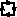
\includegraphics{cwplaqsub.pdf}}}}


\def\su2{\textsl{SU}(2)}
\def\o3{\textsl{O}(3)}
\def\uone{\textsl{U}(1)}
\def\u2{\textsl{U}(2)}
\def\CL{\textsl{CL}}
\def\CR{\textsl{CR}}
\def\CU{\textsl{CU}}
\def\CAv{\mathbf{Int}}
\def\gl2c{\textsl{GL}(2, \mathbb{C})}
\def\lasu2{\mathfrak{su}(2)}
\def\lauone{\mathfrak{u}(1)}


\newtheorem{theorem}{Theorem}[section]
\newtheorem{lemma}[theorem]{Lemma}
\newtheorem{corollary}[theorem]{Corollary}

\theoremstyle{definition}
\newtheorem{definition}[theorem]{Definition}
\newtheorem{example}[theorem]{Example}

\theoremstyle{remark}
\newtheorem{remark}[theorem]{Remark}

\numberwithin{equation}{section}

\begin{document}
%\bibliographystyle{amsplain}

\title[TNS for lattice gauge theory]{Tensor network states for lattice gauge theory}

\author{Ashley Milsted}
\address{Leibniz Universit\"at Hannover, Institute of Theoretical Physics, Appelstra{\ss}e 2, D-30167 Hannover, Germany}
\author{Tobias J.\ Osborne}
\address{Leibniz Universit\"at Hannover, Institute of Theoretical Physics, Appelstra{\ss}e 2, D-30167 Hannover, Germany}
\email{tobias.osborne@itp.uni-hannover.de}

\date{\today}

\begin{abstract}
	We study a class of locally gauge invariant tensor network quantum states for quantum lattice gauge theories in the hamiltonian formalism. 
\end{abstract}

\maketitle

\section{Introduction}

Nonabelian gauge theory is a fundamental component of the standard model of particle physics describing the dynamics of all known subatomic particles. Pure gauge theory, known as Yang-Mills theory, has been at the focus of a tremendous amount of effort in the past decades. Thanks to asymptotic freedom we now have a rather satisfactory understanding of the high-energy limit of Yang-Mills theory via perturbation theory. However, the non-perturbative infrared limit relevant for observable physics has resisted complete solution.

The most successful tool so far in the study of Yang-Mills theory and the standard model has been the computer. When quantum field theory is regulated (after a Wick rotation) on a space-time lattice \cites{wilson:1974b, creutz:1985a} the intractable path integral representation becomes amenable to Monte Carlo sampling. This approach has lead to unparalleled insights culminating in the recent determination of the hadronic spectrum of QCD \cite{duerr:2008a}. 

However, the success of Monte Carlo methods in the study of Yang-Mills theory and the standard model is not entirely satisfactory. Vast computational effort is required to obtain nonperturbative results relevant for predictions because, e.g., the smallest lattices required involve hundreds of thousands of sites and therefore very large numbers of samples are required to reduce statistical errors. The brute-force approach of lattice gauge theory theory is also somewhat at odds with our aesthetic hopes for a ``satisfactory'' understanding. Many believe that the  symmetry of Yang-Mills theory should result in a succinct explanation of its low-energy physics. These dreams are best summarised by a quote of Polyakov\footnote{http://quantumfrontiers.com/2012/12/11/fundamental-physics-prize-prediction-polyakov/.}: \begin{quote} QCD must be exactly soluble, or else I cannot imagine what the physics textbooks of the future will look like. \end{quote} The search for a simpler explanation of the low-energy physics of Yang-Mills theory prompts us to consider approaches other than Monte Carlo.

One setting where an alternative to Monte Carlo has been successful is that of \emph{quantum spin systems} in condensed matter physics \cites{auerbach:1994a, sachdev:2011a}. Here the variational method, combined with expressive variational classes, has proved to be a powerful tool in our understanding of strongly correlated physics. These variational approaches fall under the rubric of the \emph{density matrix renormalisation group} (DMRG) \cites{schollwoeck:2005a,schollwock:2011a} and have led to remarkable insights in recent years providing new tools to overcome many previously insurmountable roadblocks such as the simulation of dynamics \cites{vidal:2003a, haegeman:2011b} and fermions \cites{corboz:2009a, corboz:2010a, corboz:2010b, kraus:2010a} without sign problems and the determination of spectral information \cite{haegeman:2012a}. These developments are due, in no small part, to new impetus from quantum information theory in the understanding of \emph{quantum entanglement}. With new entanglement-inspired variational classes known as \emph{tensor networks}, including the projected entangled-pair states (PEPS) \cite{verstraete:2004a} and the multiscale entanglement renormalisation ansatz (MERA) \cites{vidal:2006a, vidal:2007a}, there has been major progress in our understanding of strongly correlated phenomena.

The MERA variational class is a sophisticated generalisation of Kadanoff's block spin renormalisation group \cite{kadanoff:1966a} which explicitly keeps track of quantum correlations discarded during a block renormalisation. Although, in a certain sense, PEPS and MERA are equivalent, there are several features of the MERA class which more easily afford analytic argumentation \cite{vidal:2009a}. Firstly, being a generalisation of the Kadanoff block-spin RG, it allows the derivation of scaling laws. Secondly, by taking account of quantum entanglement in a hierarchical way, MERA exhibit entropy area laws crucial for the description of local quantum physics. Thirdly, the causal structure of the MERA tensor network allows for an economical calculation of correlation functions. Finally, as we explain in an appendix to this paper, the MERA structure naturally emerges in the scaling limit of any quantum system approaching a quantum phase transition.

There are now several crucial hints that MERA might be a powerful tool in the study of lattice gauge theory because the ground state space of $\mathbb{Z}/2\mathbb{Z}$-lattice gauge theory (and quantum double models) admits an exact description as a MERA \cite{aguado:2008a} (this construction was later generalised to string-net models \cite{buerschaper:2009a, koenig:2009a}). This construction has been  supplemented with numerical results \cite{tagliacozzo:2011a} strongly indicating the utility of the MERA ansatz in the description of the low-energy physics of lattice gauge theories. These results strongly suggest that an economic description of the low-energy limit of Yang-Mills theory might be found in MERA.

There are still many challenges facing the hypothesis that MERA might be useful for the solution of Yang-Mills theory: there is still a large gap between the discrete gauge groups so far considered these MERA investigations and the compact gauge groups $\su2$ and $\textsl{SU}(3)$ relevant for the standard model. Additionally, there is not yet any systematic way to take a continuum limit of a MERA to obtain a representation of Wightman functions required for a quantum field description. (A continuum generalisation of MERA is available \cite{haegeman:2011a}, but it doesn't seem well suited for locally gauge-invariant quantum fields.)

In this paper we pursue a description of the ground-state of lattice gauge theory in terms of a MERA tensor network. We work with pure gauge theory in the hamiltonian formalism \cite{kogut:1975a} on the lattice and study the locally gauge invariant sector of hilbert space. We develop a toolkit to describe states in this sector, exploiting parallel transport operations and block-spin averaging operations to construct hierarchical tensor networks. This paper is intended as a high-level overview of a program: the results here, while only described at a heuristic level, are eventually intended to be lifted to the level of mathematical rigour. 

There have been several notable mathematical approaches to the study of Yang-Mills theory. We mention, in particular, three programs. All three of these approaches rely, in various ways, upon the renormalisation group \cite{wilson:1975a} and path-integral type formalisms in terms of action functionals on spacetime. The first program \cites{balaban:1985a,balaban:1988a,balaban:1984a,balaban:1984b,balaban:1985b,balaban:1985c,balaban:1985d,balaban:1989a,balaban:1989b,balaban:1987a,balaban:1988b}, due to Ba{\l}aban studies the behaviour of the partition function for lattice gauge theory under the action of block-spin renormalisation operations. This unfortunately incomplete program has yielded important successes, resulting in a proof of the ultraviolet stability of the partition function \cite{balaban:1985d} in three spacetime dimensions. Similar to Ba{\l}aban, the second program \cites{federbush:1987a,federbush:1986a,federbush:1987b,federbush:1987c,federbush:1988a,federbush:1990a}, due to Federbush, establishes that the continuum limit of the Yang-Mills field is determined by an inductive limit of block-spin renormalisations. Again, unfortunately, this program is incomplete as the construction of the Schwinger or Wightman functionals for the theory was not obtained.  The final approach \cite{magnen:1993a} studies pure Yang-Mills in the continuous case, but in the presence of an infrared cutoff. Here the existence of pure Yang-Mills theory is proved and the associated Schwinger functionals constructed. The limit where the cutoff is removed was not considered.


\section{Overview}
There are a variety of approaches for studying quantum gauge theories, originating from the possible choices of regulator and gauge fixing. According to the choice of regulator and gauge fixing different properties of the quantum theory are harder or easier to prove. For example, we can choose to maintain or break lorentz invariance, break local gauge invariance, break a manifestly local description, etc. It seems to be impossible to simultaneously maintain Lorentz invariance, local gauge invariance, a local description, and a space with a positive-definite inner product. Thus we must choose to give up on at least one of these four desiderata. 

Our choices in this paper are dictated by the desire to maintain exact local gauge invariance at all stages and to work with an explicit positive hilbert space throughout. The easiest way (in view of our constructions) to maintain local gauge invariance is to use a lattice regulator \cite{wilson:1974b, creutz:1985a}. In order to work with a manifestly positive inner-product space we exploit the temporal or Weyl gauge and work in the hamiltonian formalism of Kogut and Susskind \cite{kogut:1975a}. 

By working with a lattice we break lorentz invariance, which is inevitable whenever working in a regulated hamiltonian setting. Thus the main task of our argument will be to take the continuum limit in such a way that lorentz invariance is restored for the resulting ground-state representation.
 
The key to our argument is the construction of a sequence of states for the lattice which are: (1) explicitly locally gauge invariant; and (2) have an explicitly controllable lengthscale, the correlation length. This construction is a generalisation of a representation developed for lattice gauge theories with discrete gauge groups \cite{aguado:2008a}. In a sense, the construction we present here is a MERA generalisation of the Migdal-Kadanoff block renormalisation procedure \cite{migdal:1975a, migdal:1975b, kadanoff:1976a, kadanoff:1977a}. 


Once we've constructed this sequence we argue that they are a good ground-state ansatz for the Kogut-Susskind hamiltonian in that they are the exact ground state for a lattice gauge hamiltonian which differs from the Kogut-Susskind hamiltonian only in the ultraviolet. The next step is to extract a continuum limit from this sequence: we achieve this by constructing an explicit representation of the quantum field operators for the electric and magnetic fields. This representation is necessarily nonlocal; the representation of the gauge field is via extended field Wilson lines \cite{summers:2012a}.

The arguments described throughout are not presented at the level of mathematical rigour as we rely on a certain amount of physical intuition to abbreviate the presentation. However, every step of the argument is rigourisable and we supply an appendix outlining the techniques required to elevate the argument to a mathematically sound level. The mathematical elaboration of the arguments in this paper will be presented elsewhere. 

\section{Preliminaries}

\subsection{Graph theory}
Our constructions pertain, throughout, to \emph{graphs}.
\begin{definition}
A \emph{graph} is an ordered pair $(V, E)$ comprising a set $V$ of vertices and a set $E$ of \emph{directed edges} which are ordered pairs $(v,w)$ of elements of $V$. A directed edge $e = (v,w)$ connects its \emph{source vertex} $v \equiv e_-$ with its \emph{target vertex} $w = e_+$. 
\end{definition}

Sometimes it is convenient to adopt a functional notation for directed edges: suppose that $e=(v,w)$ is an edge, then we dually think of $e$ as a function which produces from the source vertex the target according to $e(v) = w$.
 
\begin{definition}
	An \emph{oriented graph} is a graph $(V, E)$ such that at most one of $(v,w)$ and $(w,v)$ is in $E$.
\end{definition}

\begin{definition}
	A \emph{path} $\gamma$ in a graph is a sequence $(e_1, e_2, \ldots, e_n)$ of edges which connect a sequence $(v_1, v_2, \ldots, v_{n+1})$ of vertices. By ``connect" in this context we mean that \emph{either} $e_j = (v_j, v_{j+1})$ \emph{or} $e_j = (v_{j+1}, v_{j})$,  $\forall j \in [n]$, where $[n] = \{1,2, \ldots, n\}$. The \emph{length} of a path $\gamma$ is equal to the number of edges in $\gamma$. Here $v_1$ is the source of the path and $v_{n+1}$ the target. We sometimes write $v\sim_\gamma w$ to indicate that there is a path $\gamma$ with $v$ its source and $w$ its target. 
\end{definition}
Thus,  $v\sim_\gamma w$ means that $v$ and $w$ are connected \emph{when all the orientations on the edges are neglected}.

\begin{remark}
A path $\gamma$ of length $n$ in a graph $(V,E)$ may be interpreted as a map $\gamma: [n] \rightarrow E$.
\end{remark}


\begin{definition}
	Suppose that $\gamma$ is a path of length $n$ in an oriented graph $(V,E)$. The \emph{sign} of the $j$th edge $e_j = \gamma(j)$ in $\gamma$, denoted $\sgn_\gamma(e_j)$, is equal to $+1$ if the edge $e_j$ is traversed in the direction corresponding to the orientation of $e_j$ and $-1$ if $e_j$ is traversed in the reverse direction.
\end{definition}

\begin{remark}
	Consider the path $\gamma$ below which connects vertices $v_1, v_2, v_3, \ldots,$ etc.
\begin{center}
	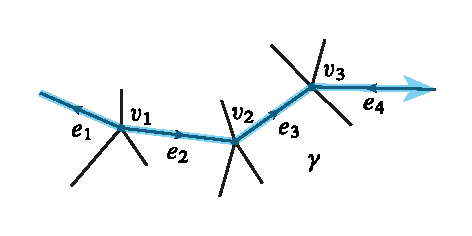
\includegraphics{path.pdf}
\end{center} 
We have that $\sgn_\gamma(e_1) = -1$, $\sgn_\gamma(e_2) = +1$, $\sgn_\gamma(e_3) = +1$, and $\sgn_\gamma(e_4) = -1$, etc.

\end{remark}

\subsection{Group theory}
We work with quantum degrees of freedom whose \emph{position variable} is an element of a compact group $G$. Informally the ``position basis'' for such a degree of freedom is written as  
\begin{equation}
	|g\rangle, \quad g\in G,
\end{equation}
with ``inner product''
\begin{equation}
	\langle g|h\rangle = \delta(g-h).
\end{equation}
Formally we work with a hilbert space $\mathcal{H} \cong L^2(G)$ whose elements may be represented as
\begin{equation}
	|\psi\rangle = \int dg\, \psi(g)|g\rangle,
\end{equation}
where $dg$ is the Haar measure.

We exploit a crucial basic result from group theory, namely,
\begin{theorem}[Peter-Weyl]
	Let $G$ be a compact group. 
	\begin{enumerate} 
	\item Then the linear span of the matrix coefficients of all finite-dimensional irreducible unitary representations of  $G$ is dense in $L^2(G)$. 
	\item Let $\{t^l\}_l$ be a maximal set of mutually inequivalent irreducible unitary representations of $G$ and let $\{t_{jk}^l(g)\}_{j,k,l}$ denote the matrix coefficients of $t^l$ in an orthonormal basis. Then $\{\sqrt{d_l} t_{jk}^l(g)\}_{j,k,l}$ is an orthonormal basis for $L^2(G)$, where $d_l$ is the dimension of $t^l$.
	\end{enumerate}
\end{theorem}
The Peter-Weyl theorem shows that $L^2(G)$ may be decomposed as
\begin{equation}
	L^2(G) \cong \bigoplus_{l} V_l\otimes V_l^*,
\end{equation}
where $V_l$ denotes the vector space furnishing the representation $t^l$ and $V^*_l$ its dual.

In the sequel, we specialise to the nonabelian case of $G \cong \su2$
and the abelian case of $G \cong \uone$. This serves to illustrate the simplifications
that can be made in the abelian case.

\subsection{The nonabelian case}
We begin with $G\cong \su2$:
\begin{equation}
	\su2 = \left\{\begin{pmatrix} \alpha & -\overline{\beta} \\ \beta & \overline{\alpha}\end{pmatrix}\,\middle|\, \alpha,\beta\in \mathbb{C}, |\alpha|^2+|\beta|^2 = 1\right\}.
\end{equation}
In this case the irreducible unitary representations are labelled by non-negative half integers, $l \in \frac12\mathbb{Z}^+$, and $d_l = 2l+1$.
We exploit the notation
\begin{equation}
	|j\rangle_l|k\rangle_l \cong \sqrt{2l+1} t_{jk}^l,
\end{equation}
for the basis $\{\sqrt{2l+1} t_{jk}^l(g)\}_{j,k,l}$, and write the scalar product as
\begin{equation}
	\langle \phi|\psi\rangle = \sum_{l}\sum_{j,k = -l}^l \overline{\widehat{\phi}_{jk}^l}\widehat{\psi}_{jk}^l,
\end{equation}
where 
\begin{equation}
	|\phi\rangle = \sum_{l}\sum_{j,k=-l}^l\widehat{\phi}_{jk}^l |j\rangle_l|k\rangle_l,
\end{equation}
and the summations over $j$ and $k$ are taken in integer steps from $-l$ to $l$. The numbers $\widehat{\phi}_{jk}^l$ are the \emph{fourier coefficients} of $\phi:G\rightarrow \mathbb{C}$, and are determined by
\begin{equation}
	\widehat{\phi}_{jk}^l = {_l\langle jk|\phi\rangle} = \sqrt{2l+1}\int dg \, \overline{t^l_{jk}}(g) \phi(g).
\end{equation}

Define the \emph{position observables} $\widehat{u}_{jk}$ via
\begin{equation}
	\widehat{u}_{jk}|g\rangle \equiv t_{jk}^{\frac12}(g)|g\rangle,
\end{equation} 
for $j,k \in \{-\frac12, \frac12\}$, i.e., $\widehat{u}_{jk}$ simply gives the matrix elements of the spin-$1/2$ representation of $g$.

The group $\su2$ is diffeomorphic to the $3$-sphere $S^3$ because of the constraint that $|\alpha|^2 + |\beta|^2 = 1$ for $\left(\begin{smallmatrix}\alpha & -\overline{\beta} \\ \beta & \overline{\alpha} \end{smallmatrix}\right) \in \su2$. 

Let $\tau^\mu$, $\mu= 0, 1, 2, 3$, denote the basis where
\begin{equation}
	\tau^0 =\begin{pmatrix}1 & 0 \\ 0 & 1\end{pmatrix}, \quad \tau^1 = {i}\begin{pmatrix} 0& 1\\ 1 & 0\end{pmatrix}, \quad \tau^2 = i\begin{pmatrix} 0& -i\\ i & 0\end{pmatrix}, \quad \text{and} \quad \tau^3 = {i}\begin{pmatrix} 1 & 0\\ 0 & -1\end{pmatrix},
\end{equation}
respectively. Note that
\begin{equation}
	(\tau^{\mu},\tau^{\nu}) = 2\delta^{\mu\nu}, 
\end{equation}
where $(A,B) \equiv \tr(A^\dag B)$.

Because $\tau^{\mu}$ is a basis for $M_2(\mathbb{C})$ we can expand $U\in \su2$:
\begin{equation}
	U = \sum_{\mu=0}^3 u_\mu \tau^\mu.
\end{equation}
Note that, for $U = \left(\begin{smallmatrix}\alpha & -\overline{\beta} \\ \beta & \overline{\alpha} \end{smallmatrix}\right) \in \su2$, the coefficients are given by $u_0 = \text{Re}(\alpha)$, $u_1 = \text{Im}(\beta)$, $u_2 = -\text{Re}(\beta)$, and $u_3 = \text{Im}(\alpha)$, so that the constraint $|\alpha|^2 + |\beta|^2 = 1$ reads
\begin{equation}
	\sum_{\alpha=0}^3 u_\alpha^2 = 1.
\end{equation}


There are several important operations on $\mathcal{H}\cong L^2(\su2)$. The first are the left and right rotations
\begin{equation}
	R_g|h\rangle \equiv |hg^{-1}\rangle, \quad \text{and}\quad L_g|h\rangle \equiv |gh\rangle, \quad g, h \in G.
\end{equation}
One can show that both $R_g$ and $L_g$ are unitary operations on $\mathcal{H}$ and that $[L_g, R_h] = 0$ for all $g,h\in G$. Note that $R_{g^{-1}} = R_{g}^{-1}$ and $L_{g^{-1}} = L_{g}^{-1}$. We also define 
\begin{equation}
	\Delta_{g} \equiv L_gR_g.
\end{equation}
The adjoint relation gives $(L_g|h\rangle)^\dag = \langle gh| = \langle h| L_g^\dag$, so that, e.g., $\langle g^{-1}h| = \langle h| L_g$. Similarly, $(R_g|h\rangle)^\dag = \langle hg^{-1}| = \langle h| R_g^\dag$, so that, e.g., $\langle hg| = \langle h| R_g$.


The matrices $\tau^1$,  $\tau^2$, and $\tau^3$ give a basis for the Lie algebra $\lasu2$ of \su2:
\begin{equation}
	[\tau^1, \tau^2] = -2\tau^3, \quad [\tau^2, \tau^3] = -2\tau^1, \quad \text{and} \quad [\tau^3, \tau^1] = -2\tau^2.
\end{equation}
We can represent these generators on $L^2(G)$ as follows. Consider the infinitesimal left rotation by $e^{\epsilon \tau^\alpha}$:
\begin{equation}
	\widehat{\ell}^\alpha_{L}|\psi\rangle \equiv \frac{d}{d\epsilon} L_{e^{\epsilon \tau^\alpha}}\Big|_{\epsilon=0}|\psi\rangle = \frac{d}{d\epsilon}\int dg \, \psi(g) | e^{\epsilon \tau^\alpha}g\rangle \Big|_{\epsilon=0}=  \int dg \, \frac{d}{d\epsilon}\psi(e^{-\epsilon \tau^\alpha}g)\Big|_{\epsilon=0} | g\rangle.
\end{equation}
Thus we have, on $L^2(G)$, that infinitesimal left rotations along $\tau^\alpha$ are represented by the differential operators
\begin{equation}
	\tau^\alpha \mapsto \widehat{\ell}^\alpha_L[\psi] \equiv  \frac{d}{d\epsilon}\psi(e^{-\epsilon \tau^\alpha}\cdot)\Big|_{\epsilon=0}.
\end{equation}
In terms of the basis $|jk\rangle_l$ the differential operators $\widehat{\ell}^\alpha_L$ act as follows
\begin{equation}
	\begin{split}
		{_l\langle jk|}\widehat{\ell}^\alpha_L|j'k'\rangle_{l'} &= \sqrt{(2l+1)(2l'+1)}\int dg\,   \overline{t^l_{jk}}(g)\frac{d}{d\epsilon} t_{j'k'}^{l'}(e^{-\epsilon \tau^\alpha}g)   \\
	 &= \sqrt{(2l+1)(2l'+1)}\int dg\,   \overline{t^l_{jk}}(g)\frac{d}{d\epsilon} t_{j'm}^{l'}(e^{-\epsilon \tau^\alpha})t_{m k'}^{l'}(g) \\
	 &= \frac{d}{d\epsilon} t_{j'm}^{l'}(e^{-\epsilon \tau^\alpha}) \delta_{jm}\delta_{kk'}\delta_{ll'}.
	\end{split}
\end{equation}
Similarly, we obtain for the infinitesimal right rotation by $e^{\epsilon \tau^\alpha}$:
\begin{equation}
	\widehat{\ell}^\alpha_{R}|\psi\rangle \equiv \frac{d}{d\epsilon} R_{e^{\epsilon \tau^\alpha}}\Big|_{\epsilon=0}|\psi\rangle = \frac{d}{d\epsilon}\int dg \, \psi(g) | ge^{-\epsilon \tau^\alpha}\rangle \Big|_{\epsilon=0}=  \int dg \, \frac{d}{d\epsilon}\psi(ge^{\epsilon \tau^\alpha})\Big|_{\epsilon=0} | g\rangle.
\end{equation}
The matrix elements of $\widehat{\ell}^\alpha_{R}$ are given by
\begin{equation}
	\begin{split}
		{_l\langle jk|}\widehat{\ell}^\alpha_R|j'k'\rangle_{l'} &= \sqrt{(2l+1)(2l'+1)}\int dg\,   \overline{t^l_{jk}}(g)\frac{d}{d\epsilon} t_{j'k'}^{l'}(ge^{\epsilon \tau^\alpha})   \\
	 &= \sqrt{(2l+1)(2l'+1)}\int dg\,   \overline{t^l_{jk}}(g) t_{j'm}^{l'}(g)\frac{d}{d\epsilon}t_{m k'}^{l'}(e^{\epsilon \tau^\alpha}) \\
	 &= \frac{d}{d\epsilon} t_{mk'}^{l'}(e^{\epsilon \tau^\alpha}) \delta_{jj'}\delta_{km}\delta_{ll'}.
	\end{split}
\end{equation}

We have the casimir element 
\begin{equation}
	\triangle = \sum_{\alpha = 1}^3 (\widehat{\ell}_L^{\alpha})^2 =  \sum_{\alpha = 1}^3 (\widehat{\ell}_R^{\alpha})^2
\end{equation}

\subsection{The abelian case}

In the abelian case of $G \cong \uone$ with
\begin{equation}
   \uone = \left\{ z \middle| z = e^{i\theta}, -\pi \le \theta < \pi \right\},
\end{equation}
which is the rotation group of a circle, there are many simplifications to be made. 
$L^2(G)$ are functions $\phi(\theta)$
such that $\langle \phi | \phi \rangle = \frac{1}{2\pi}\int_{-\pi}^{\pi} d\theta \overline{f(\theta)} f(\theta)$ is
finite. The irreducible representations of $\uone$ are
the familiar fourier modes $z^n(\theta) = e^{in\theta}$ with $n \in \mathbb{Z}$.
They are all one-dimensional so that there is only a single matrix coefficient
for each $n$. We use the notation
\begin{equation}
  |n\rangle \cong e^{in\theta}
\end{equation}
so that we may decompose functions as
\begin{equation}
  |\phi\rangle = \sum_n \widehat{\phi}^n |n\rangle,
\end{equation}
where $\hat{\phi}^n$ are the fourier coefficients of $\phi(\theta)$
given by
\begin{equation}
  \widehat{\phi}^n = \langle n|\phi\rangle = \frac{1}{2\pi} \int_{-\pi}^{\pi} d\theta \, e^{-in\theta} \phi(\theta).
\end{equation}
We may write scalar products using the fourier coefficients as
\begin{equation}
  \langle \phi|\psi\rangle = \sum_n \overline{\widehat{\phi}^n} \widehat{\psi}^n.
\end{equation}

We further define a position observable $\widehat{u}$ so that
\begin{equation}
  \widehat{u}|g\rangle = e^{i\theta} |g\rangle.
\end{equation}

The Lie algebra $\lauone$ consists of the antihermitian $1 \times 1$ matrices.
A basis is given by the imaginary unit $i$ and an infinitesimal rotation has the 
form $e^{i\epsilon}$. Setting $g = e^{i\epsilon}$ we obtain the 
infinitesimal left rotation
\begin{equation}
  \widehat{\mathcal{l}}_L |\psi\rangle \equiv \frac{d}{d\epsilon} \left. L_{e^{i\epsilon}} \right|_{\epsilon = 0} |\psi\rangle
    = \frac{d}{d\epsilon} \int_{-\pi}^{\pi} \left. \frac{d\theta}{2\pi} \psi(\theta) |\theta + \epsilon\rangle \right|_{\epsilon = 0}
    = \frac{d}{d\epsilon} \int_{-\pi}^{\pi} \left. \frac{d\theta}{2\pi} \psi(\theta - \epsilon) \right|_{\epsilon = 0} |\theta\rangle
\end{equation}
and the infinitesimal right rotation
\begin{equation}
  \widehat{\mathcal{l}}_R |\psi\rangle \equiv \frac{d}{d\epsilon} \left. R_{e^{i\epsilon}} \right|_{\epsilon = 0} |\psi\rangle
    = \frac{d}{d\epsilon} \left. \int_{-\pi}^{\pi} \frac{d\theta}{2\pi} \psi(\theta) |\theta - \epsilon\rangle \right|_{\epsilon = 0}
    = \frac{d}{d\epsilon} \left. \int_{-\pi}^{\pi} \frac{d\theta}{2\pi} \psi(\theta + \epsilon) \right|_{\epsilon = 0} |\theta\rangle
\end{equation}
On $L^2(G)$ we thus have corresponding differential operators
\begin{equation}
  i \mapsto \widehat{\mathcal{l}}_L[\psi](\theta) \equiv \left. \frac{d}{d\epsilon} \psi(\theta - \epsilon) \right|_{\epsilon = 0}
    = - \psi'(\theta),
\end{equation}
\begin{equation}
  i \mapsto \widehat{\mathcal{l}}_R[\psi](\theta) \equiv \left. \frac{d}{d\epsilon} \psi(\theta + \epsilon) \right|_{\epsilon = 0}
    = \psi'(\theta).
\end{equation}
As noted above, a left rotation $L_g$ is just the inverse
of the right rotation $R_g$.

The matrix elements of $\widehat{\mathcal{l}}_L$ and $\widehat{\mathcal{l}}_R$
in terms of the $|n\rangle$ basis are
\begin{equation}
  \langle n|\widehat{\mathcal{l}}_L |m\rangle = \int_{-\pi}^{+\pi} \frac{d\theta}{2\pi}
    e^{-in\theta} \frac{d}{d\epsilon} e^{im(\theta - \epsilon)} \bigg|_{\epsilon = 0}
    = -in\delta_{nm},
\end{equation}
\begin{equation}
  \langle n|\widehat{\mathcal{l}}_R |m\rangle = \int_{-\pi}^{+\pi} \frac{d\theta}{2\pi}
    e^{-in\theta} \frac{d}{d\epsilon} e^{im(\theta + \epsilon)} \bigg|_{\epsilon = 0}
    = in\delta_{nm}.
\end{equation}
\section{Controlled gates}
In this section we describe the fundamental operations we exploit in the construction of gauge-invariant tensor network states. 

The basic building block of our constructions is the \emph{controlled rotation}: given a unitary representation $U$ of $G$ on a vector space $V$ we define the operation
\begin{equation}
	\CU \equiv \int dg\, |g\rangle\langle g| \otimes U(g),
\end{equation}
on $L^2(G)\otimes V$. The first tensor factor is called the \emph{control} and the second factor the \emph{target}. When $\CU$ acts on a multipartite system $W\otimes \mathcal{H}_c\otimes V_t\otimes W'$ we use the notation
\begin{equation}
	\CU_{ct} \equiv \mathbb{I}_W\otimes \CU\otimes \mathbb{I}_{W'}
\end{equation}
to indicate which tensor product factors $\CU$ acts on.

In the particular case where $U(g) \equiv L_g$ or $U(g) \equiv R_g$ we obtain the controlled left and right rotations defined by
\begin{equation}
	\textsl{CL} \equiv \int dg\, |g\rangle \langle g| \otimes L_g, \quad\text{and}\quad \CR \equiv \int  dg\,|g\rangle \langle g| \otimes R_g,
\end{equation}
which are unitary operations on $L^2(G\times G)$:
\begin{equation}
	\langle \CL\phi, \CL \psi\rangle = \int dg_1dg_2\, \overline{\phi}(g_1,g_1^{-1}g_2) \psi(g_1, g_1^{-1}g_2) = \langle \phi, \psi\rangle.
\end{equation}
It turns out that $\CL$ and $\CR$ intertwine rotations in an interesting way:
\begin{equation}
	\begin{split}
		(L_g \otimes \mathbb{I})  \CL &= \int dh\, |gh\rangle \langle h| \otimes L_{h} \\
		&= \int dh'\, |h'\rangle \langle g^{-1}h'| \otimes L_{g^{-1}h'} \\
		&= (\mathbb{I}\otimes L_g^\dag) \CL  (L_g\otimes \mathbb{I}),\\
	\end{split}
\end{equation}
\begin{equation}
	\begin{split}
		\CL (\mathbb{I} \otimes L_g) &= \int dh\, |h\rangle \langle h| \otimes L_{h}L_g \\
		&= \int dh'\, |h'g^{-1}\rangle \langle h'g^{-1}| \otimes L_{h'} \\
		&= (R_g \otimes \mathbb{I}) \CL  (R_g^\dag\otimes \mathbb{I}),\\
	\end{split}
\end{equation}
\begin{equation}
	\begin{split}
		(L_g \otimes L_g)  \CL &= \int dh\, |gh\rangle \langle h| \otimes L_{gh} \\
		&= \int dh'\, |h'\rangle \langle g^{-1}h'| \otimes L_{h'} \\
		&= \CL  (L_g\otimes \mathbb{I}).\\
	\end{split}
\end{equation}
and
\begin{equation}
	\begin{split}
		(R_g \otimes R_g)  \CL &= \int dh\, |hg^{-1}\rangle \langle h| \otimes L_{h}R_{g} \\
		&= \int dh'\, |h'\rangle \langle h'g| \otimes L_{h'}L_{g}R_{g} \\
		&= \CL  (R_{g}\otimes L_g R_g).\\
	\end{split}
\end{equation}
From which we learn that
\begin{equation}
	\begin{split}
	\CL(L_g\otimes \mathbb{I}) \CL^\dag &= L_g \otimes L_g \\ 
	\CL(R_g\otimes L_g) \CL^\dag &= R_g\otimes \mathbb{I}\\
	\CL  (R_{g}\otimes L_g R_g)\CL^\dag &= R_g \otimes R_g \\
	\CL  (\mathbb{I}\otimes R_g )\CL^\dag &= \mathbb{I} \otimes R_g \\
	\end{split}
\end{equation}


The action of the controlled-rotation gates on the position operators may be calculated as follows.
In the case of $G\cong \su2$:
\begin{equation}
	\begin{split}
		\CL^\dag ( \widehat{u}_{jk}\otimes \mathbb{I} )\CL|g\rangle|h\rangle &= t_{jk}^{\frac12}(g)|g\rangle |h\rangle = ( \widehat{u}_{jk}\otimes \mathbb{I} )|g\rangle|h\rangle, \\
		\CL^\dag ( \mathbb{I}\otimes \widehat{u}_{jk}  )\CL|g\rangle|h\rangle &= \sum_{j'=-\frac12}^{\frac12}t_{jj'}^{\frac12}(g)t_{j'k}^{\frac12}(h)|g\rangle |h\rangle = \sum_{j'=-\frac12}^{\frac12}( \widehat{u}_{jj'}\otimes \widehat{u}_{j'k} )|g\rangle|h\rangle, \\
		\CR^\dag ( \widehat{u}_{jk}\otimes \mathbb{I} )\CR|g\rangle|h\rangle &= t_{jk}^{\frac12}(g)|g\rangle |h\rangle = ( \widehat{u}_{jk}\otimes \mathbb{I} )|g\rangle|h\rangle, \\
		\CR^\dag ( \mathbb{I}\otimes \widehat{u}_{jk}  )\CR|g\rangle|h\rangle &= \sum_{j'=-\frac12}^{\frac12}t_{jj'}^{\frac12}(h)\overline{t}_{kj'}^{\frac12}(g)|g\rangle |h\rangle = \sum_{j'=-\frac12}^{\frac12}( \widehat{u}_{kj'}^\dag\otimes \widehat{u}_{jj'} )|g\rangle|h\rangle. \\
	\end{split}
\end{equation}
For $G\cong \uone$, the final results are the same except that there are no 
indices on the position operators.

\section{Gauge theory on a graph}
In this section we introduce the main object of our study, namely, \emph{gauge theories on graphs}. Here we largely follow the formulation of Baez \cite{baez:1996a}.

Let $(V,E)$ be an oriented graph. Our gauge theories are principle $G$-bundles $P$ over the vertex space $V$ with the discrete topology. Since such structures are trivialisable we fix a trivialisation from the outset. This allows us to describe $P$ as follows. We attach, to each edge $e$, the classical position coordinate $G$, so that classical configurations of our system correspond to elements of
\begin{equation}
	\mathcal{A} = \prod_{e\in E} G.
\end{equation}
The set $\mathcal{A}$ is the space of \emph{connections} on the graph $(V,E)$. The \emph{gauge transformations} of $(V,E)$ are given by
\begin{equation}
	\mathcal{G} = \prod_{v\in V} G.
\end{equation}
The group $\mathcal{G}$ acts on $\mathcal{A}$ by
\begin{equation}
	(xA)_e = x_{e_-} A_e x_{e_+}^{-1},
\end{equation}
where $A_e$ denotes the component of $A \in \mathcal{A}$ associated with the edge $e$ and, similarly, $x_v$ denotes the component of $x\in \mathcal{G}$ associated with vertex $v$ 


The quantum degree of freedom we associate with each edge is then the hilbert space $L^2(G)$. Thus the total hilbert space for our system is
\begin{equation}
	\mathcal{H} = \bigotimes_{e\in E} \mathcal{H}_e.
\end{equation}
For $G \cong \su2$ we visualise the state $|\psi\rangle_e$ of a single edge as follows
\begin{center}
	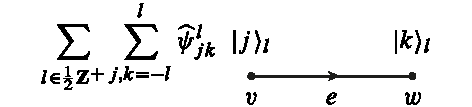
\includegraphics{edgespace.pdf}.
\end{center}
Note that this visualisation is slightly misleading in the case where $G$ is 
abelian or has more than a single one-dimensional irreducible representation.
The case of $G \cong \uone$ has both these properties: It is abelian and all
irreducible representations are one-dimensional, so that 
acting from the left is the same as acting from the right and we 
may simply associate the state 
$|\psi\rangle_e = \sum_{n\in \mathbb{Z}} \widehat{\psi}^n |n\rangle_e$
with the complete edge $e$.

We henceforth associate the left tensor factor in the direct sum for $\mathcal{H}_e$ with the source vertex $v = e_-$  and the right tensor factor with the target vertex $w = e_+$. (As we'll see, this identification is congruent with the action of the local gauge group $\mathcal{G}$.) Thus, each vertex $v$ in the graph $(V,E)$ is associated with the left and right factors of $\mathcal{H}_e$ for each edge incident with $v$, as in the following diagram.
\begin{center}
	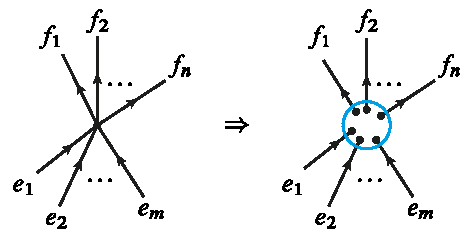
\includegraphics{vertexspace.pdf}
\end{center}

\begin{definition}
	Let $(V,E)$ be an oriented graph and $\mathcal{H}$ the total hilbert space of connections. The \emph{gauge group} $\mathcal{G}$ is represented on $\mathcal{H}$ by 
	\begin{equation}
		\pi(x) = \bigotimes_{e\in E} L_{x_{e_-}}R_{x_{e_+}}, \quad x\in \mathcal{G}.
	\end{equation}
\end{definition}

\subsection{Classical parallel transport}
The classical notion of parallel transport through a gauge field on a graph may be described as follows. Suppose that we have an object transforming according to a representation $U$ of $G$. We think of the object as living at some vertex $v$. Whenever the object moves to another vertex $w$ along a path $\gamma$ it undergoes the \emph{parallel transport}  
\begin{equation}\label{eq:ugamma}
	U(\gamma) \equiv \prod_{e\in \gamma} U(g_{e}^{-\sgn_\gamma{e}}),
\end{equation}
where the product is taken from \emph{right to left}.

\begin{example}
Consider the path $\gamma$ in the oriented graph:
\begin{center}
	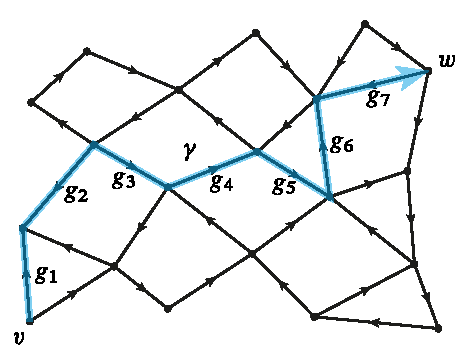
\includegraphics{paralleltx.pdf}
\end{center}
The parallel transport associated with the path $\gamma$ from $v$ to $w$ is given by
\begin{equation}
	U(\gamma) = U(g_{7})U(g_{6}^{-1})U(g_{5}^{-1})U(g_{4}^{-1})U(g_{3}^{-1})U(g_{2}) U(g_{1}^{-1}).
\end{equation}
\end{example}
Under a gauge transformation $A \mapsto xA$, a parallel transporter $U(\gamma)$ transforms as
\begin{equation}
	U(\gamma) \underset{x\in \mathcal{G}}{\longmapsto} U(x_{w}^{-1}) U(\gamma) U(x_{v}).
\end{equation}

\subsection{Quantum parallel transport}
The quantum representation of the parallel transport is furnished by the controlled rotation operation $\CU$: let $\gamma$ be a path in $(V,E)$ and denote by
\begin{equation}
	\begin{split}
		\CU_\gamma &\equiv \int \left(\prod_{e\in \gamma} dg_e\right)\,  \left(\bigotimes_{e\in \gamma} |g_e\rangle\langle g_e|\right) \otimes U(\gamma), \\
		&= \prod_{e\in \gamma} {\CU_{e s}}^{-\sgn_\gamma{e}}
	\end{split}
\end{equation}
where the product is taken, as usual, from right to left, and $U(\gamma)$ is defined as in (\ref{eq:ugamma}). It is clear that $\CU_\gamma$ is an \emph{entangling} operation and, hence, there is no way in general to separate the gauge degrees of freedom from a quantum particle's position degree of freedom as it undergoes parallel transport: these two degrees of freedom will typically become strongly entangled during parallel transport.

Because a vertex may be regarded as a quantum particle we can exploit parallel transport to move vertices (and their associated edges) around the gauge network. This operation is effected by using for the representation $U(g)$ either the left and right multiplication operations $L_g$ or $R_g$ as follows. Suppose we wish to move the target vertex $v = f_+$ of an edge $f \in E$ to some other vertex $w$ along a path $\gamma$. Then we simply need to apply the operation
\begin{equation}
	\CR_\gamma \equiv \prod_{e\in \gamma} {\CR_{e f}}^{-\sgn_\gamma{e}}
\end{equation}
In the following example we illustrate the parallel transport of the target vertex of the edge $f$ from vertex $v$ to $w$.
\begin{center}
	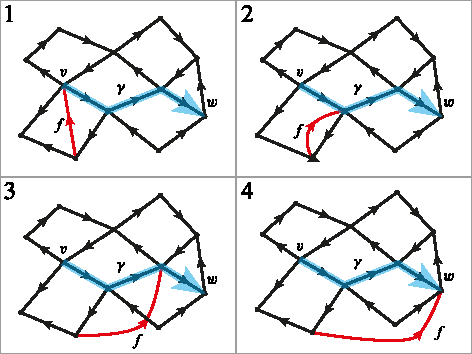
\includegraphics{edgetx.pdf}
\end{center}
Note that planarity of the graph $(V,E)$ is not relevant for this operation: the procedure is identical for any oriented graph.


\section{The gauge-invariant subspace}
We are interested in the gauge-invariant subspace of $\mathcal{H}$ which is the subspace spanned by all vectors satisfying
\begin{equation}
	\pi(x) |\psi\rangle = |\psi\rangle, \quad \forall x \in \mathcal{G}.
\end{equation}

The most important gauge-invariant state is the one built from the trivial representation of $G$ in $L^2(G)$. This state is denoted $|0\rangle$ and is given by
\begin{equation}
	|0\rangle = \int dg\, |g\rangle.
\end{equation}
This state is simply the basis vector $|00\rangle_0 \cong t^0_{00}(g)$ for $G \cong \su2$
or $|0\rangle \cong z^0(\theta)$ for $G \cong \uone$. 
Note that left and right invariance of the haar measure means that
\begin{equation}
	L_x|0\rangle = R_x|0\rangle = |0\rangle, \quad \forall x \in G.
\end{equation}
Using $|0\rangle$ we can build the gauge-invariant state 
\begin{equation}
	|\Omega_0\rangle = \bigotimes_{e\in E} |0\rangle.
\end{equation}

Another important gauge-invariant state is that of a \emph{loop} consisting of a single vertex and a single edge:
\begin{center}
	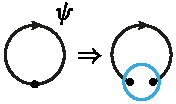
\includegraphics{singlevertex.pdf}
\end{center}
Here the total hilbert space is simply $\mathcal{H}$. The local gauge group $\mathcal{G} \cong G$ acts as
\begin{equation}
	|\psi\rangle \mapsto L_xR_x |\psi\rangle, \quad \forall x\in G.
\end{equation}
Thus a state $|\psi\rangle$ is gauge invariant if and only if
\begin{equation}\label{eq:classstate}
	\int dg\, \psi(g) |g\rangle= \int dg\, \psi(g) |xgx^{-1}\rangle = \int dg\, \psi(x^{-1}gx) |g\rangle, \quad\forall x\in G.
\end{equation}
That is, $\psi$ must be a \emph{class function}, $\psi(x^{-1}gx) = \psi(g)$. 
For abelian $G$ such as $G \cong \uone$ we have $x^{-1}gx = g \quad \forall x,g \in G$ so that all
such states are gauge invariant.

Gauge invariant states such as $|\psi\rangle$ enjoy the useful property that the expectation values of many operators significantly simplify. For example
\begin{equation}
	\begin{split}
	\langle \widehat{\ell}_L^j\rangle =\frac{d}{d\epsilon}\langle \psi|L_{e^{i\epsilon \sigma^j}}|\psi\rangle\bigg|_{\epsilon = 0} &= \frac{d}{d\epsilon}\langle \psi|L_x^\dag R_x^\dag L_{e^{i\epsilon \sigma^j}} L_x R_x|\psi\rangle\bigg|_{\epsilon = 0} \\
	&= \frac{d}{d\epsilon}\langle \psi|  L_{x^\dag e^{i\epsilon \sigma^j}x}  |\psi\rangle\bigg|_{\epsilon = 0} \\
	&= \frac{d}{d\epsilon}\langle \psi|  L_{ e^{i\epsilon x^\dag\sigma^jx}}  |\psi\rangle\bigg|_{\epsilon = 0} \\
	&= \frac{d}{d\epsilon}\langle \psi|  L_{ e^{i\epsilon \sum_{k} O_{jk}\sigma^k}}  |\psi\rangle\bigg|_{\epsilon = 0} \\
	&= \sum_{k} O_{jk}\langle \widehat{\ell}_L^k\rangle,
	\end{split}
\end{equation}
where $O_{jk}$ are the matrix elements of an arbitrary $\o3$ rotation. Since this is true for all $O\in \o3$ we conclude that $\langle \widehat{\ell}_L^j\rangle = 0 = \langle\widehat{\ell}_R^j\rangle$, for all $j=1, 2, 3$. Similarly
\begin{equation}
	[C]_{jk} \equiv \langle \widehat{\ell}_L^j \widehat{\ell}_L^k\rangle = \sum_{j'k'} O_{jj'}O_{kk'}\langle \widehat{\ell}_L^{j'} \widehat{\ell}_L^{k'}\rangle = [OCO^T]_{jk},
\end{equation}
for all $O\in \o3$. As a consequence of Schur's lemma we then conclude that 
\begin{equation}
	C = c\mathbb{I},
\end{equation}
that is, $\langle \widehat{\ell}_L^j \widehat{\ell}_L^k\rangle = c\delta_{jk}$.


\section{The Kogut-Susskind hamiltonian}
Remarkably the dimension of the gauge-invariant sector does not scale with number of edges, but rather with the number of noncontractible loops. Thus the allowed configuration space for a cycle graph is near trivial. However, the gauge-invariant sector for graphs in two dimensions and above is a very high-dimensional space and there are many nontrivial microscopic models one could write down. A crucial requirement of any microscopic model for Yang-Mills theory is that its continuum limit is Lorentz invariant. An important class of microscopic model, due to Kogut and Susskind, has been argued to give a Lorentz invariant continuum limit \cite{kogut:1975a}:
\begin{equation}
	H = \frac{g^2}{2 a} \sum_{e\in E} \widehat{\ell}^2_e - \frac{2}{g^2 a} \sum_{\square} \text{Re}(\tr(\widehat{u}_{\cwplaqsub})).
\end{equation}

\section{Tensor networks for gauge invariant states}
Using the trivial state $|\Omega_0\rangle$, gauge invariant loops, and parallel transportation, we can build arbitrary gauge-invariant quantum states via the processes of \emph{edge subdivision} and \emph{edge addition}.

\subsection{Edge subdivision}
An edge in a gauge-invariant state of our graph bundle may be subdivided as follows. Suppose that $|\psi\rangle$ is a gauge-invariant state for an oriented graph bundle $(V,E)$ and we wish to subdivide an edge $e = (v,w)$. Then we obtain a new gauge-invariant state for the oriented graph bundle $(V',E')$ where $V' = V\cup \{v'\}$ and $E' = (E\setminus \{e\} )\cup\{ (v,v'), (v',w)\}$ using the procedure:
\begin{enumerate}
	\item Adjoin an ancillary subsystem in the state $|0\rangle_{e'}$, where $e' = (v,v')$, resulting in the new state
	\begin{equation}
		|\psi\rangle |0\rangle_{e'}.
	\end{equation} 
	\item Apply $\CL^{-1}$ to glue the new edge to the end of the old edge $e$:
	\begin{equation}
		\CL_{e' e}^{-1}|\psi\rangle |0\rangle_{e'}.
	\end{equation}
	\item Relabel the subsystem $e$ as $e'' = (v',w)$. We end up with the state
	\begin{equation}
		|\psi'\rangle = \int d\mathbf{g}dg_{e'}dg_{e''} \, \psi(\mathbf{g},g_{e''}) |\mathbf{g}\rangle |g_{e'}\rangle_{e'}  |g^{-1}_{e'}g_{e''}\rangle_{e''},
	\end{equation}
\end{enumerate}
where $\mathbf{g}$ refer to the connection variables attached to edges in $E\setminus \{e\}$.
The edge subdivision procedure is simply a parallel transport of the source vertex of $e$ along a new edge $e'$ initialised in the trivial state $|0\rangle$:
\begin{center}
	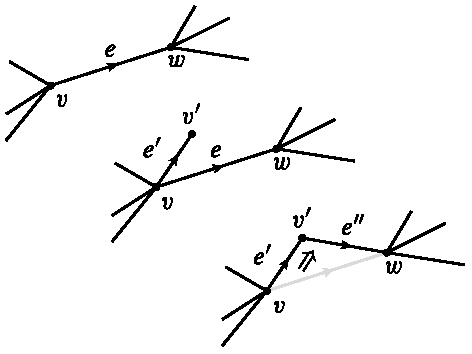
\includegraphics{edgesubdivide.pdf}
\end{center}

We now prove that any state produced by edge subdivision is locally gauge invariant. Since the only subsystems involved in an edge subdivision are $e'$ and $e''$ we need only check the invariance of $|\psi'\rangle$ under gauge transformations acting on the vertices $v, v'$, and $w$: 
\begin{equation}
	\pi(x) \equiv \cdots \otimes L_{x_{e_-'}}R_{x_{e_+'}}\otimes L_{x_{e_-''}}R_{x_{e_+''}} \otimes \cdots;
\end{equation}
for clarity we write $x \equiv x_{e_-'}$, $y \equiv x_{e_+'} = x_{e_-''}$, and $z \equiv x_{e_+''}$. Thus we see, after some changes of variable, that
\begin{equation}
	\begin{split}
	( \cdots \otimes L_{x}R_{y}\otimes L_{y}R_{z} \otimes \cdots)|\psi'\rangle &= \int d\mathbf{g}dg_{e'}dg_{e''} \, \psi(\mathbf{g},g_{e''}) |\mathbf{g}'\rangle |xg_{e'}y^{-1}\rangle_{e'}  |yg^{-1}_{e'}g_{e''}z^{-1}\rangle_{e''} \\
	&= \int d\mathbf{g}dg_{e'}dg_{e''} \, \psi(\mathbf{g},g_{e''}) |\mathbf{g}'\rangle |g_{e'}\rangle_{e'}  |g^{-1}_{e'}xg_{e''}z^{-1}\rangle_{e''} = |\psi'\rangle.
	\end{split}
\end{equation}

\subsection{Edge addition}
The addition of an edge (in a product state) proceeds similarly to edge subdivision. To add an edge $f = (v,w)$ between two vertices $v$ and $w$ we add a loop to a vertex $v$ initialised in a gauge invariant state $|\phi\rangle$ and parallel transport the target (or the source) vertex along a path $\gamma$ connecting $v$ and $w$ to its destination vertex $w$.  Concretely the procedure is as follows:
\begin{enumerate}
	\item Adjoin an ancillary subsystem in the state $|\phi\rangle_{f}$ of the form (\ref{eq:classstate}):
	\begin{equation}
		|\psi\rangle |\phi\rangle_{f}.
	\end{equation} 
	\item Apply $\CR_\gamma$ to parallel transport the target vertex to $w$. The final result is
	\begin{equation}
		|\psi'\rangle = \CR_{\gamma}|\psi\rangle |\phi\rangle_{f}.
	\end{equation}
\end{enumerate}

In contrast to the case of edge subdivision, the state $|\psi'\rangle$ resulting from edge addition generally depends on the path along which the target vertex of $f$ is parallel transported.

\section{Gauge connection interpolation}
In this section we study a process whereby edges are added to faces of an oriented graph in as flat a way as possible. There are considerable similarities between the methods proposed here and the block-spin renormalisations of Ba{\l}aban and Federbush and the \emph{link smearing} of Morningstar and Peardon \cite{Morningstar:2004a}.

\subsection{Subdividing a face}\label{subsec:facesubd}
Consider the lattice gauge interpolation problem: we have two vertices $v$ and $w$ and two edges $e_1$ and $e_2$ from $w$ to $v$ with a gauge connection $U$ and $V$ on each edge, respectively. Suppose we add a third edge $e_3$ from $w$ to $v$ between $e_1$ and $e_2$, setting its gauge connection $W$ in such a way that the two newly formed plaquettes are as flat as possible. This means that we want to find $W = \mathbf{I}(U,V)\in \su2$ such that $UW^\dag$ and $WV^\dag$ are both as close to the identity as possible and such that if we subject the lattice to a local gauge transformation then $W$ transforms in the correct way. That is, if $U\mapsto xUy^\dag$ and $V\mapsto xVy^\dag$ then $\mathbf{I}(xUy^\dag,xVy^\dag)= x\mathbf{I}(U,V)y^\dag$.
\begin{center}
	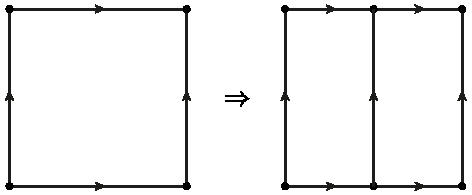
\includegraphics{facesubdivision.pdf}
\end{center}

Here we claim that the solution to this problem may be found variationally as follows: consider
\begin{equation}\label{eq:wmin}
	\ell(U,V) \equiv \min_{W\in \su2} \|W-U\|_2^2 + \|W-V\|_2^2,
\end{equation}
where
\begin{equation}
	\|A\|_2^2 = \frac{1}{2}\tr(A^\dag A).
\end{equation}
It is clear that if $\mathbf{I}(U,V)$ is a minimiser for (\ref{eq:wmin}) then $x\mathbf{I}(U,V)y^\dag$ is a minimiser for the case where $U$ and $V$ are subjected to $U\mapsto xUy^\dag$ and $V\mapsto xVy^\dag$.


The expression involved in the minimisation is equal to
\begin{equation}
	\begin{split}
		\|W-U\|_2^2 + \|W-V\|_2^2 &= \frac12 \tr( (W-U)^\dag (W-U) ) + \frac12 \tr((W-V)^\dag (W-V)) \\
		&= 4 - \frac12\tr(W^\dag(U+V)) - \frac12\tr(W(U^\dag+V^\dag)) \\ 
		&= 4-\text{Re}[\tr(W^\dag(U+V))].
	\end{split}
\end{equation}
Thus, defining $A = U+V$, we are reduced to solving the following maximisation problem
\begin{equation}
	\max_{W\in \su2} \text{Re}[\tr(W^\dag A)],
\end{equation}
for general $A$.

We now provide an expression for the unique maximiser. To do this we exploit the formula
\begin{equation}\label{eq:mat_param_exp}
	e^{i\alpha \mathbf{u}\cdot \paulivec} = \cos(\alpha)\mathbb{I} + i\sin(\alpha) \mathbf{u}\cdot \paulivec,
\end{equation} 
where 
\begin{equation}
	\paulivec \equiv \left[ \left(\begin{smallmatrix} 0 & 1 \\ 1 & 0\end{smallmatrix}\right),\left(\begin{smallmatrix} 0 & -i \\ i & 0\end{smallmatrix}\right), \left(\begin{smallmatrix} 1 & 0 \\ 0 & -1\end{smallmatrix}\right) \right],
\end{equation}
and $\alpha\in [0,2\pi)$ and $\|\mathbf{u}\|_2 = 1$. Notice that 
\begin{equation}
	\cos(\alpha) = \frac12\tr(U) \quad \text{and} \quad \sin(\alpha) = \pm\sqrt{1-\frac14\tr(U)^2},
\end{equation} 
and 
\begin{equation}
	i \mathbf{u}\cdot \paulivec = \pm\frac{U-\frac12\tr(U)\mathbb{I}}{\sqrt{1-\frac14\tr(U)^2}}.
\end{equation} 
	In the case
\begin{equation}
	A = A_0\mathbb{I} + i\mathbf{a}\cdot \paulivec,
\end{equation}
with $\mathbf{a}\in \mathbb{R}^3$, we can write our maximisation problem as
\begin{equation}
	2\max_{\substack{\gamma\in[0,2\pi)\\ \|\mathbf{w}\|_2=1}} \left(\cos(\gamma) A_0 + \sin(\gamma)(w_x a_x + w_y a_y+ w_z a_z)\right).
\end{equation}
Now the answer to this is straightforward: choose 
\begin{equation}
	\mathbf{w} = \frac{\mathbf{a}}{\|\mathbf{a}\|_2},
\end{equation}
and
\begin{equation}
	\cos(\gamma) = \frac{A_0}{\sqrt{A_0^2 + \|\mathbf{a}\|_2^2}} = \frac{A_0}{\|A\|_2},
\end{equation}
i.e.,
\begin{equation}
	\gamma = \cos^{-1}\left(\frac{A_0}{\|A\|_2}\right).
\end{equation}

Now we calculate $A_0$ and $\mathbf{a}$ for our problem. Write
\begin{equation}
	U = e^{i\alpha \mathbf{u}\cdot \paulivec}, \quad \text{and} \quad V = e^{i\beta \mathbf{v}\cdot \paulivec}.
\end{equation}
Note that 
\begin{equation}
	A_0 = \frac12 \tr(U+V),
\end{equation}
and
\begin{equation}
	i\mathbf{a}\cdot\boldsymbol{\sigma} = U-\frac12\tr(U)\mathbb{I} + V-\frac12\tr(V)\mathbb{I}.
\end{equation}
Exploiting (\ref{eq:mat_param_exp}) we find
\begin{equation}
	A_0 = \cos(\alpha) + \cos(\beta), \quad \text{and}\quad \mathbf{a} = \sin(\alpha)\mathbf{u} + \sin(\beta)\mathbf{v}.
\end{equation}
We obtain, for the maximiser $W$, the expression
\begin{equation}
	\mathbf{I}(U,V) = e^{i\gamma \mathbf{w}\cdot \paulivec} = e^{i\cos^{-1}\left(\frac{A_0}{\|A\|_2}\right) \frac{\mathbf{a}\cdot\paulivec}{\|\mathbf{a}\|_2}} = \frac{A_0}{\|A\|_2}\mathbb{I} + i\sqrt{1-\frac{A_0^2}{\|A\|_2^2}}\frac{\mathbf{a}\cdot\paulivec}{\|\mathbf{a}\|_2}
\end{equation}
which simplifies to
\begin{equation}
	\mathbf{I}(U,V) = \frac{1}{\|A\|_2}\left[ A_0\mathbb{I} + i\mathbf{a}\cdot\paulivec \right]
	 = \frac{U+V}{\sqrt{\frac12\tr[(U+V)^\dag(U+V)]}}.
\end{equation}
Note that $\mathbf{I}(U,V) = \sqrt{VU^\dag} U$. This can be confirmed by multiplying $\frac{U+V}{\sqrt{\frac12\tr[(U+V)^\dag(U+V)]}}$ by $U^\dag \sqrt{UV^\dag}$.

\subsubsection{Subdividing a face into $n$ pieces}
Here we generalise the calculation for the optimal face subdivision to the case where we add $n-1$ edges in as flat a way as possible. Pictorially this task is illustrated as follows:

\begin{center}
	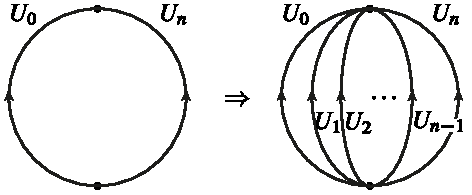
\includegraphics{facemsection.pdf}
\end{center}

The solution may be again found variationally: consider
\begin{equation}
	\ell(U_0, U_{n}) = \min_{U_1, \ldots, U_{n-1} \in \su2} \sum_{j=0}^{n-1} \|U_j-U_{j+1}\|_2^2 = 4n - 2\min_{U_1, \ldots, U_{n-1} \in \su2} \sum_{j=0}^{n-1}  \text{Re}\tr(U_j^\dag U_{j+1}).
\end{equation}
We are free to multiply our solution $(U_0, U_1, \ldots, U_{n})$ from the left by $U_0^\dag$ followed by a conjugation by any $\eta\in\su2$: thus, as long as we can solve the subdivision problem for $V_0 = \mathbb{I}$ and $V_{n} = e^{i\phi \sigma^z}$, we can use this to find the general solution by exploiting $\eta$ given by $\eta U_0^\dag U_{n} \eta^\dag = e^{i\phi \sigma^z}$.


Writing
\begin{equation}
	U_j = \sum_{\mu} u_\mu(j)\tau^\mu
\end{equation}
this becomes a purely geometric problem in one dimension:
\begin{equation}
	\ell(U_0, U_{n}) = 4n - 2 \min_{u(1), \ldots, u(n-1) \in S^1}  \sum_{j=0}^{n-1}\sum_{\mu} u_\mu(j)u_\mu(j+1),
\end{equation}
where 
\begin{equation}
	u(j) = \begin{pmatrix} \cos(\phi_j) \\ 0 \\ 0 \\ \sin(\phi_j)\end{pmatrix},
\end{equation}
with $\phi_0 = 0$ and $\phi_{n} = \phi$ (we assume that $\phi <\pi$),
so that
\begin{equation}
	\ell(U_0, U_{n}) = 4n - 2 \min_{\phi_1, \ldots, \phi_{n-1}}  \sum_{j=0}^{n-1}\sum_{\mu} \cos(\phi_j-\phi_{j+1}).
\end{equation}
The solution is given by
\begin{equation}
	\phi_j = \frac{j\phi}{n},
\end{equation}
whence
\begin{equation}
	V_j = e^{i\frac{j\phi}{n} \sigma^z}
\end{equation}
and
\begin{equation}
	U_j = U_0 \eta^\dag V_j \eta = U_0 (U_0^\dag U_{n})^{\frac{j}{n}}.
\end{equation}

\subsubsection{Interpolate a face from $m$ to $n$ pieces}
Here we apply the method from the previous subsection to take a face which is already subdivided into $m$ pieces and interpolate or resample it into $n$ pieces with $n>m$. We carry out this procedure in two steps. First we subdivide each of the $m$ faces into $n$ pieces according to previously described method and then we resample the face. 

The configuration of the $m$-fold subdivided face is specified by
\begin{equation}
	(U_0, U_1, \ldots, U_{m}).
\end{equation}
We now subdivide each face $(U_{j},U_{j+1})$ into $n$ pieces by adding $n-1$ edges $V_{j,k}$,   according to the rule
\begin{equation}
	\begin{split}
		V_{j,0} &\equiv U_j \\
		V_{j,1} &\equiv U_j (U_j^\dag U_{j+1})^{\frac{1}{n}} \\
			&\vdots \\
		V_{j,n-1} &\equiv U_j (U_j^\dag U_{j+1})^{\frac{n-1}{n}}. \\
	\end{split}
\end{equation}
Then we resample to obtain the new assignment
\begin{equation}
	\begin{split}
		U_0' &= V_{0,0} \\
		U_1' &\equiv V_{0,m}\\
		U_2' &\equiv V_{\lfloor\frac{2m}{n}\rfloor,2m - \lfloor\frac{2m}{n}\rfloor n}\\
			&\vdots \\
		U_{n-1}'&\equiv V_{m-1,n-m}\\
		U_{n}' &\equiv U_m. \\
	\end{split}
\end{equation}
The most interesting case in the sequel is where $n= m+1$, in which case we find
\begin{equation}
	U_j' = U_{j}(U_{j}^\dag U_{j-1})^{\frac{j}{m+1}}, \quad j = 0,1, 2, \ldots, m.
\end{equation}

We now consider the case where $n\rightarrow \infty$. Set $\epsilon = 1/n$ and introduce the ``position'' variable $x = j\epsilon$. We now write 
\begin{equation}
	U(x) \equiv U_{\lfloor x/\epsilon \rfloor}.
\end{equation}
Thus we write, for the interpolated unitaries,
\begin{equation}
	U'(x) = U(x)(U(x)^\dag U(x-\epsilon))^{\frac{x}{1+\epsilon}}.
\end{equation}
Writing $U(x-\epsilon) \equiv U(x)(\mathbb{I}-i\epsilon K(x)) + O(\epsilon^2)$ we find
\begin{equation}
	U'(x) = U(x)(\mathbb{I}-i\epsilon K(x))^{\frac{x}{1+\epsilon}}.
\end{equation}




\subsection{Plaquette subdivision}

Suppose we have a plaquette in a planar oriented graph bundle $(V,E)$. We study the task of subdividing the plaquette and the corresponding connection $g_e$ into subplaquettes in as ``flat'' a way as possible:
\begin{center}
	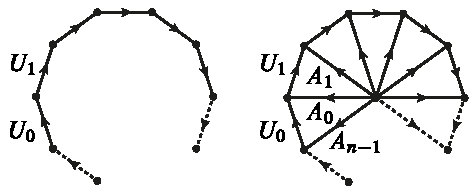
\includegraphics{plaquettesubdivision.pdf}
\end{center}
To this end we study the problem of minimising the curvature of connection of the subdivided plaquette:
\begin{equation}
	E(A_0, \ldots, A_{n-1}; U_0, \ldots, U_{n-1}) = \max_{A_j\in \su2} \sum_{j=0}^{n-1} \text{Re}(\tr(U_j A_j^\dag A_{j-1})),
\end{equation}
where $n\equiv 0\, (\text{mod}\, n)$ and $U_j\in \su2$, $j=0, 1, \ldots, n-1$. When written in terms of the expansions $A_j = \sum_{\mu} a_\mu(j) \tau^{\mu}$ we find
\begin{equation}
	E = \max_{a_\mu(j)\in S^3} \sum_{j=0}^{n-1}\sum_{\mu,\nu = 0}^3 a_\mu(j)\text{Re}(\tr(U_j (\tau^{\mu})^\dag \tau^\nu))a_\nu(j-1)
\end{equation}
We add lagrange multipliers to enforce the constraints that $a_\mu(j)\in S^3$:
\begin{equation}
	L = \max_{a_\mu(j)\in S^3} \sum_{j=0}^{n-1}\sum_{\mu,\nu = 0}^3 a_\mu(j)\text{Re}(\tr(U_j (\tau^{\mu})^\dag \tau^\nu))a_\nu(j-1) + \sum_{j=0}^{n-1}\sum_{\mu = 0}^3 \lambda_j a_\mu(j)^2.
\end{equation}
The extrema of $L$ are determined by
\begin{equation}
	-2\lambda_j a_\mu(j) = \sum_{\nu = 0}^3\text{Re}(\tr(U_j (\tau^{\mu})^\dag \tau^\nu))a_\nu(j-1) + a_\nu(j+1)\text{Re}(\tr(U_{j+1} (\tau^{\nu})^\dag \tau^\mu)).
\end{equation}
These equations may be expressed in a more direct matrix form:
\begin{equation}
	-2\lambda_j A_j = 2\sum_{\mu = 0}^3 (\tau^{\mu}, A_{j-1}U_j)\tau^\mu + (A_{j+1}U_{j+1}^\dag, \tau^\mu ) \tau^\mu =2 A_{j-1}U_j+ 2A_{j+1}U_{j+1}^\dag.
\end{equation}
This expression may then, in turn, be compactly expressed as follows
\begin{equation}
	Mv = \Lambda v,
\end{equation}
where
\begin{equation}
	v = \sum_{j=0}^{n-1} |j\rangle \otimes A_j^\dag,
\end{equation}
\begin{equation}
	\Lambda = -\sum_{j=0}^{n-1}  \lambda_j|j\rangle\langle j|\otimes\mathbb{I},
\end{equation}
and
\begin{equation}
	M = \sum_{j=0}^{n-1} |j+1\rangle\langle j| \otimes U_{j+1}^\dag + |j-1\rangle\langle j|\otimes U_{j}.
\end{equation}

All eigenvectors of a matrix of the form $M$ have the following form
\begin{equation}
	|\psi_{\pm}(k)\rangle = \frac{1}{\sqrt{n}}\sum_{j=0}^{n-1} e^{-i\frac{j\phi_{\pm}}{n}}\mu^{jk}|j\rangle \otimes U_{j}^\dag\cdots U_0^\dag |\eta_{\pm}\rangle,
\end{equation}
where $U_{n-1}^\dag U_{n-2}^\dag \cdots U_0^\dag |\eta_{\pm}\rangle = e^{i\phi_{\pm}}|\eta_{\pm}\rangle$. Consider the action of $M$ on $|\psi_{\pm}(k)\rangle$:
\begin{equation}
	\begin{split}
	M|\psi_{\pm}(k)\rangle &= \frac{1}{\sqrt{n}}\sum_{j=0}^{n-1}\left\{ e^{-i\frac{j\phi_{\pm}}{n}}\mu^{jk}|j+1\rangle \otimes U_{j+1}^\dag U_{j}^\dag \cdots U_0^\dag |\eta_{\pm}\rangle + e^{-i\frac{j\phi_{\pm}}{n}}\mu^{jk}|j-1\rangle \otimes U_{j-1}^\dag \cdots U_0^\dag |\eta_{\pm}\rangle \right\} \\
	&=\frac{1}{\sqrt{n}}\sum_{j=0}^{n-1}\left\{ e^{-i\frac{(j-1)\phi_{\pm}}{n}}\mu^{(j-1)k}|j\rangle \otimes U_{j}^\dag \cdots U_0^\dag |\eta_{\pm}\rangle + e^{-i\frac{(j+1)\phi_{\pm}}{n}}\mu^{(j+1)k}|j\rangle \otimes U_{j}^\dag\cdots U_0^\dag |\eta_{\pm}\rangle \right\} \\
	&=\frac{1}{\sqrt{n}}\sum_{j=0}^{n-1}\left(e^{i\frac{\phi_{\pm}}{n}}\mu^{-k} + e^{-i\frac{\phi_{\pm}}{n}}\mu^{k}\right )\left\{ e^{-i\frac{j\phi_{\pm}}{n}}\mu^{jk}|j\rangle \otimes U_{j}^\dag\cdots U_0^\dag |\eta_{\pm}\rangle \right\} \\
	&= 2\cos\left(\frac{\phi_{\pm} -2\pi k}{n}\right)|\psi_{\pm}(k)\rangle.
	\end{split}
\end{equation}
The phase $\phi_+$ is related to $\phi_-$ via $\phi_- = 2\pi - \phi_+$. Hence, the eigenvalues of $M$ are doubly degenerate and are given by
\begin{equation}
	\lambda(k) = 2\cos\left(\frac{\phi_{+} -2\pi k}{n}\right), \quad k = 0, 1, \ldots, n-1,
\end{equation}
with corresponding eigenvector pairs
\begin{equation}
	\{|\psi_{+}(k)\rangle, |\psi_{-}(1-k)\rangle\}.
\end{equation}
Using these eigenvector pairs we can construct elements of $\su2$ as follows. Let 
\begin{equation}\label{eq:interpespaces}
	V_j(k) = \begin{pmatrix} e^{-i\frac{j\phi_{+}}{n}}\mu^{jk}U_{j}^\dag \cdots U_0^\dag |\eta_{+}\rangle & \Big| & e^{-i\frac{j\phi_{-}}{n}}\mu^{j(1-k)}U_{j}^\dag\cdots U_0^\dag |\eta_{-}\rangle\end{pmatrix}, \quad j = 0, 1, \ldots, n-1.
\end{equation}
This expression simplifies to
\begin{equation}
	V_j(k) = U_{j}^\dag\cdots U_0^\dag  \eta \begin{pmatrix} \theta_+(j,k) & 0 \\ 0 &  \theta_-(j,k)\end{pmatrix}, \quad j = 0, 1, \ldots, n-1,
\end{equation}
where $\theta_+(j,k) = e^{-i\frac{j\phi_{+}}{n}}\mu^{jk}$ and $\theta_-(j,k) = e^{-i\frac{j\phi_{-}}{n}}\mu^{j(1-k)}$ and 
\begin{equation}
	\eta = \begin{pmatrix}  \langle 0|\eta_{+}\rangle & \langle 0|\eta_{-}\rangle \\ \langle 1|\eta_{+}\rangle & \langle 1|\eta_{-}\rangle\end{pmatrix}.
\end{equation}
Note that $\theta_+(j,k) = \theta_-^{-1}(j,k)$, so that 
\begin{equation}
	V_j(k) = U_{j}^\dag\cdots U_0^\dag  \eta \begin{pmatrix} \theta_+(j,k) & 0 \\ 0 &  \theta_+^{-1}(j,k)\end{pmatrix}, \quad j = 0, 1, \ldots, n-1,
\end{equation}
It turns out that each $V_j(k)$ is an element of $\su2$ already as the matrix $\eta$ is precisely the matrix diagonalising $U_{n-1}\cdots U_0$,
\begin{equation}
	\eta^\dag U_{n-1}^\dag\cdots U_0^\dag \eta = \begin{pmatrix} e^{i\phi_+} & 0 \\ 0 &  e^{i\phi_-}\end{pmatrix}\equiv \Phi,
\end{equation}
and hence $\eta$ may be itself chosen to be an element of $\su2$.

We thus construct $n$ possible solutions to our interpolation problem, namely,
\begin{equation}
	A_j = \theta(j,k)^\dag \eta^\dag U_0 \cdots U_{j}, \quad k = 0, 1, \ldots, n-1.
\end{equation}
With this choice we find that
\begin{equation}
	U_jA_j^\dag A_{j-1} = U_{j-1}^\dag \cdots U_0^\dag  \eta \theta(j,k)\theta(j-1,k)^\dag\eta^\dag U_0 \cdots U_{j-1},  \quad k = 0, 1, \ldots, n-1,
\end{equation}
so that
\begin{equation}
	\text{Re}(\tr(U_jA_j^\dag A_{j-1})) = \text{Re}(\tr(\theta(j,k)\theta(j-1,k)^\dag)).
\end{equation}
The interpolated curvature then becomes
\begin{equation}
	E = 2n \cos\left(\frac{\phi_+ - 2\pi k}{n}\right).
\end{equation}
Since our quantities are densities the curvature density becomes
\begin{equation}
	E = 2 \cos\left(\frac{\phi_+ - 2\pi k}{n}\right).
\end{equation}
Denoting the energy of a plaquette before the subdivision as $E' = 2\cos(\phi_+)$, we see that by inverting this equation:
\begin{equation}
	E' = \cos(n\arccos(E)) = T_n(E),
\end{equation} 
where $T_n(z)$ is the $n$th Chebyshev polynomial.

\subsection{Interpolating the cube}
To study the realistic case of Yang-Mills theory in $(3+1)$ dimensions we need to be able to perform subdivisions of $3$-dimensional cubes. Here we encounter a new complication: while the procedure still requires the solution of a linear problem it results in a generalised eigenvalue problem rather than a simple eigenvalue problem. 

Suppose we have a gauge field configuration on an elementary cube in the regular lattice $\mathbb{R}^3$. Our objective is to, as per the previous subsection, subdivide this cube into $8$ subcubes in as flat a way as possible. If we just aim to optimise the curvature over all the new edges we encounter a nonlinear optimisation problem. This doesn't completely render this problem impossible; we can still say a lot about the existence of and the properties of the solutions (more on this later).

Here we first follow a different route: we break our problem into two linear subproblems. While this may not give the globally optimal solution it will give a solution that respects the symmetries of our problem.

The first stage of our linearised approach is to subdivide the faces of the cube using our existing subdivision solution:
\begin{center}
	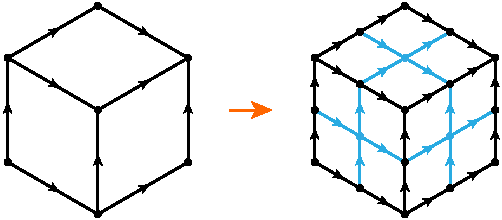
\includegraphics{cubeinterpf1.pdf}
\end{center}
The next task is to add in the interior edges:
\begin{center}
	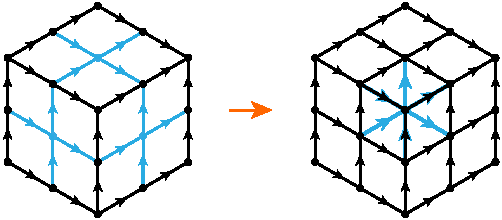
\includegraphics{cubeinterpf2.pdf}
\end{center}
We now discuss this step. Given that the connections on all the subdivided faces are fixed we can combine those relevant for the curvature of the newly added interior edges; we end up with the problem of interpolating a diamond:
\begin{center}
	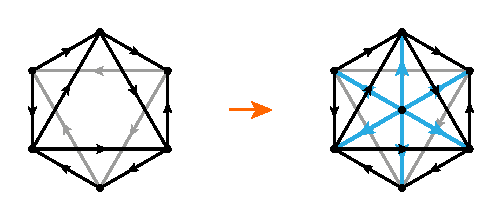
\includegraphics{diamondinterp.pdf}
\end{center}
The curvature of the new edges is proportional to
\begin{equation}
	\begin{split}
		\text{Re}\Big[	\tr(U_0 A_1^\dag B_0) + \tr(U_1 B_1^\dag A_1) &+ \tr(U_2 A_0^\dag B_1) + \tr(U_3 B_0^\dag A_0) +  \\
						\tr(V_0 A_1^\dag C_0) + \tr(V_1 C_1^\dag A_1) &+ \tr(V_2 A_0^\dag C_1) + \tr(V_3 C_0^\dag A_0) + \\
						\tr(W_0 C_1^\dag B_0) + \tr(W_1 B_1^\dag C_1) &+ \tr(W_2 C_0^\dag B_1) + \tr(W_3 B_0^\dag C_0)\Big],
	\end{split}
\end{equation}
where we've labelled the connections according to
 \begin{center}
	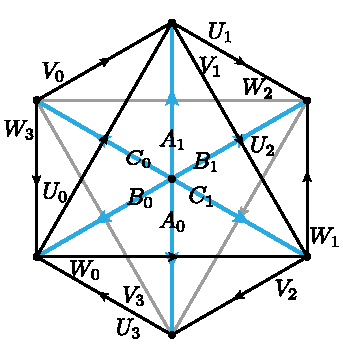
\includegraphics{diamondconn.pdf}
\end{center}



\subsection{Response to perturbations}
In this subsection we study the response of the interpolated set $A_j$ arising from a plaquette subdivision to a perturbation of one of the elements $U_j$.

Specifically, we are interested in perturbations of the form
\begin{equation}
	U_j(\epsilon) \equiv U_j e^{i\epsilon X_j},
\end{equation}
with $X^\dag_j = X_j$ and $\tr(X_j) = 0$, $j = 0, 1, \ldots, n-1$. Since we already know the general solution for $A_j$ we simply substitute this perturbation into the expression for $A_j$:
\begin{equation}
	A_j(\epsilon) = \theta(j,k; \epsilon)^\dag \eta^\dag(\epsilon) U_0(\epsilon) \cdots U_{j}(\epsilon), \quad k = 0, 1, \ldots, n-1,
\end{equation}
where 
\begin{equation}	
	\theta(j,k; \epsilon) = \begin{pmatrix} e^{-i\frac{j\phi_{+}(\epsilon)}{n}}\mu^{jk} & 0 \\ 0 &  e^{i\frac{j\phi_{+}(\epsilon)}{n}}\mu^{-jk}\end{pmatrix},
\end{equation}
with 
\begin{equation}
	U_{n-1}^\dag(\epsilon) U_{n-2}^\dag(\epsilon) \cdots U_0^\dag(\epsilon) |\eta_{\pm}(\epsilon)\rangle = e^{i\phi_{\pm}(\epsilon)}|\eta_{\pm}(\epsilon)\rangle.
\end{equation}
Note that we can obtain $\phi_+(\epsilon)$ from
\begin{equation}
	\phi_+(\epsilon) = \arccos\left(\frac12 \tr(U_{n-1}^\dag(\epsilon) U_{n-2}^\dag(\epsilon) \cdots U_0^\dag(\epsilon))\right).
\end{equation}

Actually, we are only interested in the first derivative of $A_j(\epsilon)$ evaluated at $\epsilon = 0$:
\begin{equation}
	\frac{d}{d\epsilon} A_j(\epsilon) \bigg|_{\epsilon = 0} = ?
\end{equation}
This calculation is greatly simplified upon noting that we need only calculate the response to a perturbation of $U_{n-1}$ because the general result then follows from a simple relabelling.

The first task in this calculation is to diagonalise the matrix
\begin{equation}
	e^{i\epsilon \sigma^j}U,
\end{equation}
where $U \equiv U_{n-1}^\dag U_{n-2}^\dag \cdots U_0^\dag$. We do this by working in the eigenbasis of $U$:
\begin{equation}
	U = \eta \Phi \eta^\dag
\end{equation}
Then, using the calculation detailed in Appendix~\ref{app:diagprod}, we find that
\begin{equation}
	e^{i\epsilon \sigma^1}\Phi = W_1(\epsilon) D_1(\epsilon) W_1^\dag(\epsilon),
\end{equation}
with
\begin{equation}
	\begin{split}
		D_1(\epsilon) &= e^{i\phi_+(\epsilon) \sigma^3}, \\
		W_1(\epsilon) &= \sqrt{\frac{1+x_3(\epsilon)}{2}}\begin{pmatrix} 1 & \frac{-x_1(\epsilon)+ix_2(\epsilon)}{1+x_3(\epsilon)}\\ \frac{x_1(\epsilon)+ix_2(\epsilon)}{1+x_3(\epsilon)} & 1\end{pmatrix},
	\end{split}
\end{equation}
where
\begin{equation}
	\begin{split}
		x_1(\epsilon) &= \frac{\sin(\epsilon)\cos(\phi_+)}{\sqrt{\sin^2(\epsilon) + \cos^2(\epsilon)\sin^2(\phi_+)}}\\
		x_2(\epsilon) &= \frac{\sin(\epsilon)\sin(\phi_+)}{\sqrt{\sin^2(\epsilon) + \cos^2(\epsilon)\sin^2(\phi_+)}}\\
		x_3(\epsilon) &= \frac{\cos(\epsilon)\sin(\phi_+)}{\sqrt{\sin^2(\epsilon) + \cos^2(\epsilon)\sin^2(\phi_+)}},
	\end{split}
\end{equation}
and
\begin{equation}
	\phi_+(\epsilon) = \cos^{-1}(\cos(\epsilon)\cos(\phi_+)).
\end{equation}
The first conclusion we can draw is that
\begin{equation}
	\frac{d}{d\epsilon}\phi_+(\epsilon)\bigg|_{\epsilon = 0} = 0,
\end{equation}
so that
\begin{equation}
	\frac{d}{d\epsilon} W_1(\epsilon)\bigg|_{\epsilon =0} = \frac{1}{{2}}\begin{pmatrix} 0 & -\cot(\phi)+i\\ \cot(\phi)+i & 0\end{pmatrix} = \frac{i}{2}\sigma^1 -\frac{i}{2}\cot(\phi)\sigma^2.
\end{equation}
Because
\begin{equation}
	\sigma^2 = e^{-i\frac{\pi}{4}\sigma^3}\sigma^1e^{i\frac{\pi}{4}\sigma^3}, \quad \text{and}\quad -\sigma^1 = e^{-i\frac{\pi}{4}\sigma^3}\sigma^2e^{i\frac{\pi}{4}\sigma^3}
\end{equation}
we deduce that for 
\begin{equation}
	e^{i\epsilon \sigma^2}\Phi = W_2(\epsilon) D_2(\epsilon) W_2^\dag(\epsilon),
\end{equation}
the derivative is given by
\begin{equation}
	\frac{d}{d\epsilon} W_2(\epsilon)\bigg|_{\epsilon =0} = \frac{i}{2}\sigma^2 +\frac{i}{2}\cot(\phi)\sigma^1.
\end{equation}
Finally, because $\sigma^3$ commutes with $\Phi$ we immediately conclude that
\begin{equation}
	\frac{d}{d\epsilon} W_3(\epsilon)\bigg|_{\epsilon =0} = 0.
\end{equation}

We now have enough information to calculate the general case: note that
\begin{equation}
	e^{i\epsilon \sigma^j}U = e^{i\epsilon \sigma^j}\eta \Phi \eta^\dag = \eta e^{i\epsilon \eta^\dag \sigma^j\eta} \Phi \eta^\dag,
\end{equation}
so 
\begin{equation}
	\begin{split}
	\zeta_1 \equiv \frac{d}{d\epsilon} \eta_1(\epsilon)\bigg|_{\epsilon =0} &= \frac{i}{2}\eta \left[O_{11}(\sigma^1 - \cot(\phi)\sigma^2) + O_{12}(\sigma^2 +\cot(\phi)\sigma^1) \right] \eta^\dag \\
	&= \frac{i}{2} (O_{11} + O_{12}\cot(\phi))\eta\sigma^1 \eta^\dag  + \frac{i}{2}(-O_{11} \cot(\phi) + O_{12})\eta\sigma^2 \eta^\dag  \\
	\zeta_1 \equiv\frac{d}{d\epsilon} \eta_2(\epsilon)\bigg|_{\epsilon =0} &= \frac{i}{2}\eta \left[O_{21}(\sigma^1 - \cot(\phi)\sigma^2) + O_{22}(\sigma^2 +\cot(\phi)\sigma^1) \right] \eta^\dag \\
	&= \frac{i}{2} (O_{21} + O_{22}\cot(\phi))\eta\sigma^1 \eta^\dag  + \frac{i}{2}(-O_{21} \cot(\phi) + O_{22})\eta\sigma^2 \eta^\dag \\
	\zeta_1 \equiv\frac{d}{d\epsilon} \eta_3(\epsilon)\bigg|_{\epsilon =0} &= \frac{i}{2}\eta \left[O_{31}(\sigma^1 - \cot(\phi)\sigma^2) + O_{32}(\sigma^2 +	\cot(\phi)\sigma^1) \right] \eta^\dag \\
	&= \frac{i}{2} (O_{31} + O_{32}\cot(\phi))\eta\sigma^1 \eta^\dag  + \frac{i}{2}(-O_{31} \cot(\phi) + O_{32})\eta\sigma^2 \eta^\dag. 
	\end{split}
\end{equation}
Using this information we then obtain
\begin{equation}
	\frac{d}{d\epsilon} A_j^{(1)}(\epsilon)\bigg|_{\epsilon =0} = \theta(j,k)^\dag  \zeta_1^\dag\eta \theta(j,k) A_j, \quad j = 0, 1, \ldots, n-2,
\end{equation}
and for the $j=n-1$ case:
\begin{equation}
	\frac{d}{d\epsilon} A_{n-1}^{(1)}(\epsilon)\bigg|_{\epsilon =0} = \theta(n-1,k)^\dag  \zeta_1^\dag\eta \theta(n-1,k) A_{n-1}- i\epsilon A_{n-1} \sigma^1.
\end{equation}

%Such perturbations, to first order, may be written as 
%\begin{equation}
%	\begin{split}
%	M(\epsilon) &=  \sum_{j=0}^{n-1} |j+1\rangle\langle j| \otimes U_{j+1}^\dag(\mathbb{I} - i\epsilon X_{j+1}) + |j-1\rangle\langle j|\otimes (\mathbb{I} + i\epsilon X_j)U_{j} \\
%	&= M_0 + \epsilon M_1
%	\end{split}
%\end{equation}
%where $M_0 \equiv M$, and 
%\begin{equation}
%	M_1 = i \sum_{j=0}^{n-1} -|j+1\rangle\langle j| \otimes U_{j+1}^\dag  X_{j+1} + |j-1\rangle\langle j|\otimes  X_jU_{j}.
%\end{equation}
%Note that the degeneracy of the eigenvalues of $M(\epsilon)$ in response to such a perturbation is not lifted to first order because  $U_j+i\epsilon X_jU_j$ is unitary to first order.
%
%Write $P_k(\epsilon)$ for the projection onto the $k$th eigenvalue of $M(\epsilon)$. The general theory of analytic perturbation theory ensures that $P_k(\epsilon)$ may be expanded in a convergent series:
%\begin{equation}
%	P_k(\epsilon) = P_k + \epsilon P^{(1)}_k + \cdots,
%\end{equation}
%where $P_k \equiv P_k(0)$ is the unperturbed eigenprojection.
%Write 
%\begin{equation}
%	P_k(\epsilon) = V(k)V^\dag(k)
%\end{equation}
%
%
%To apply perturbation theory to calculation the change in $A_j$ we need to account for the two-fold degeneracy in the eigenvalues of $M_0$. Thus we study the perturbation restricted to the corresponding two-dimensional eigenspaces of $M$:
%\begin{equation}
%	V^\dag (k) M_1 V(k),
%\end{equation}
%where
%\begin{equation}
%	V(k) = \sum_{j=0}^{n-1} |j\rangle \otimes V_j(k),
%\end{equation}
%and $V_j(k)$ is given by (\ref{eq:interpespaces}). We find that
%\begin{equation}
%	\begin{split}
%		V^\dag (k) M_1 V(k) &= i\sum_{j=0}^{n-1}  -V_{j+1}^\dag(k)U_{j+1}^\dag X_{j+1} V_j(k) + V_{j-1}^\dag(k)X_jU_{j} V_j(k) \\
%		&= i\sum_{j=0}^{n-1}  -\theta(j+1,k)^\dag \eta^\dag U_0\cdots U_{j} X_{j+1} U_{j}^\dag\cdots U_0^\dag  \eta \theta(j,k) + \\ &\quad \quad\theta(j-1,k)^\dag \eta^\dag U_0 \cdots U_{j-1} X_j U_{j-1}^\dag\cdots U_0^\dag  \eta \theta(j,k).
%	\end{split}
%\end{equation}
%In the case where only $X_0 \not= 0$ we find
%\begin{equation}
%	\begin{split}
%	V^\dag (k) M_1 V(k) &=-i   \eta^\dag U_0\cdots U_{n-1} X_{0} U_{n-1}^\dag\cdots U_0^\dag  \eta \theta(n-1,k)  + i\theta(n-1,k)^\dag \eta^\dag X_0   \eta \\
%	&= -i \Phi^\dag \eta^\dag X_0   \eta \Phi\theta(n-1,k)  + i\theta(n-1,k)^\dag \eta^\dag X_0   \eta. \\
%	\end{split}
%\end{equation}


\section{Wilson flow}
In this section we explore an alternative method to calculate the interpolation of a parallel transport network. This approach is based on the \emph{Wilson flow} procedure whereby the interpolating unitaries are calculated gradually via gradient descent. This technique is sufficiently general to supply us with the general solution of the interpolation problem.

\subsection{A simple example}
As a first encounter with this approach we consider the basic face subdivision problem:
\begin{equation}
	\max_{W\in \su2} \text{Re}[\tr(W^\dag A)].
\end{equation}
We could simply solve this problem via brute force, but this doesn't always work for more elaborate situation. However there is a general but more indirect method: introduce a \emph{flow parameter} $s \in \mathbb{R}^+$ and allow $W$ to depend continuously on $s$ and set up a flow equation which sends $W(s)$ to the solution as $s\rightarrow \infty$. In order to ensure that $W(s)\in\su2$ we assume that 
\begin{equation}\label{eq:wilsonflow}
	\frac{d}{ds} W(s) = i H(s) W(s),
\end{equation}
where $H(s)$ is a traceless hermitian operator. We solve for $H(s)$ by maximising the \emph{energy}
\begin{equation}
	E(s) \equiv \tr\left[W^\dag(s)A + W(s) A^\dag\right].
\end{equation}
This is achieved by solving the maximisation problem
\begin{equation}
	\begin{split}
	\max_{H(s)} \frac{d}{ds}E(s) &= \max_{H(s)} i\tr\left[H(s)W^\dag(s)A - W(s)H(s) A^\dag\right] + \lambda \tr(H^\dag(s)H(s)) \\ 
	&= \max_{H(s)} i\tr\left[H(s)(W^\dag(s)A - A^\dag W(s))\right]+ \lambda \tr(H^\dag(s)H(s))
	\end{split}
\end{equation}
Parametrising
\begin{equation}
	H(s) = \sum_{j=1}^3 h_j(s)\sigma^j,
\end{equation}
we find
\begin{equation}
	h_j(s) = \frac{1}{2\lambda} \tr\left[\sigma^j\Delta(s)\right],
\end{equation}
from which we infer that $H(s)$ is simply given by the traceless part of $\Delta(s)$, where
\begin{equation}
	\Delta(s) \equiv i(W^\dag(s)A - A^\dag W(s)).
\end{equation}
It is easy to see that the fixed point of this equation is given by
\begin{equation}
	W(s) = \sqrt{VU^\dag} U,
\end{equation}
because in this case
\begin{equation}
	\Delta = i\left( U^\dag \sqrt{U V^\dag}(U+V) - (U^\dag + V^\dag) \sqrt{VU^\dag} U \right) = 0.
\end{equation}

We now goto the general loop case:
\begin{equation}
	E(s) = \sum_{j=0}^{n-1} \text{Re}(\tr(U_j A_j^\dag(s) A_{j-1}(s)).
\end{equation}
Again we parametrise $A_j(s)$ according to
\begin{equation}
	\frac{d}{ds} A_j(s) = i H_j(s) A_j(s),
\end{equation}
where $H_j(s)$ is a traceless hermitian operator.

As before we calculate the change in the energy and enforce that the step is finite via lagrange multiplier:
\begin{equation}
	\begin{split}
	\frac{d}{ds}E(s) &= \sum_{j=0}^{n-1} \text{Re}(\tr(U_j A_j^\dag(s) (iH_{j-1}(s)-iH_j(s)) A_{j-1}(s)) + \sum_{j=0}^{n-1} \lambda_j \tr(H^\dag_j(s)H_j(s)) \\
	&= \sum_{j=0}^{n-1} \text{Re}(\tr(H_j(s)\Delta_j(s)) + \sum_{j=0}^{n-1} \lambda_j \tr(H^\dag_j(s)H_j(s)),
	\end{split}
\end{equation}
where
\begin{equation}
	\Delta_j(s) = -i A_{j-1}(s) U_j A_j^\dag(s) + i A_{j}(s) U_{j+1} A_{j+1}^\dag(s).
\end{equation}
Carrying out the maximisation gives us
\begin{equation}
	H_j(s) = \frac1{2\lambda_j}(\Delta_j(s)+\Delta_j^\dag(s)) - \frac1{4\lambda_j}\tr(\Delta_j(s)+\Delta_j^\dag(s))\mathbb{I}.
\end{equation}

This prescription generalises in a natural way to arbitrary graphs and, as we'll see in the next subsection, even allows us to carry out interpolations that would otherwise require the solution of a nonlinear equation. 

 

\subsection{Quantum Wilson flow}
Here we describe how to use the classical Wilson flow described in the previous section to arrive a quantum interpolation scheme. The main observation is that the quantum Wilson flow is essentially the classical Wilson flow: for the simple plaquette bisection case we see that
\begin{equation}
	|U\rangle |\mathbb{I}\rangle |V\rangle \mapsto |U\rangle |W(s)\rangle |V\rangle,
\end{equation}
where $W(s)$ is determined by the Wilson flow equation (\ref{eq:wilsonflow}) with initial condition $W(0) = \mathbb{I}$. We write this as a unitary operation via a controlled rotation:
\begin{equation}
	|U\rangle |W(s)\rangle |V\rangle \equiv \mathcal{U}_s |U\rangle |\mathbb{I}\rangle |V\rangle.
\end{equation}
Note that we do not obtain a unitary operator if we define a map 
\begin{equation}
	|U\rangle |W(0)\rangle |V\rangle \mapsto |U\rangle |W(s)\rangle |V\rangle,
\end{equation}
where $W(s)$ is found from Wilson flow with initial condition $W(0)$ (we need to compensate the loss of norm with an additional term).

\section{Averaged parallel transport}
In this section we exploit the gauge connection interpolation prescriptions developed in the previous section to obtain a parallel transport operation which may be interpreted as transporting a quantity according to the ``average" of the parallel transport of a given set of paths. This operation may then, in turn, be exploited to build improved tensor networks for gauge-invariant states.

\subsection{Moving between two edges}

Consider two vertices $v$ and $w$ connected by two paths $\gamma_1$ and $\gamma_2$, respectively. Here we exploit the interpolation $\mathbf{I}(U,V)$ developed in \S\ref{subsec:facesubd} to write down an averaged quantum parallel transport operation connecting $v$ to $w$. This operation is given by
\begin{equation}
	\CAv_{\gamma_1,\gamma_2} \equiv \int dUdV \, |U\rangle\langle U|\otimes |V\rangle\langle V| \otimes R_{\mathbf{I}(U,V)}^\dag,
\end{equation}
where $U$ is the connection of the path $\gamma_1$ and $V$ the connection of the path $\gamma_2$.

Let's now suppose, for simplicity, that $\gamma_1$ and $\gamma_2$ are simply edges joining $v$ and $w$, i.e., $\gamma_1 = e_1$ and $\gamma_2 = e_2$. The averaged parallel transport operation then acts on the operators $L_g$, $R_g$, and $\widehat{u}_{jk}$, in the following way:
\begin{equation}
	\begin{split}
	 (R_g\otimes \mathbb{I} \otimes \mathbb{I}) \CAv_{e_1,e_2} &= \int dUdV \, |Ug^\dag\rangle\langle U| \otimes  |V\rangle\langle V| \otimes R_{\mathbf{I}(U,V)}^\dag \\
	&= \int dU'dV \, |U'\rangle\langle U'g| \otimes  |V' g\rangle\langle V'g| \otimes R_{\mathbf{I}(U'g,V'g)}^\dag \\
	&= (\mathbb{I} \otimes R_g^\dag   \otimes R_g^\dag) \CAv_{e_1,e_2} (R_g \otimes R_g\otimes \mathbb{I}).
	\end{split}
\end{equation}
Thus 
\begin{equation}
	(R_g\otimes R_g \otimes R_g) \CAv_{e_1,e_2} = \CAv_{e_1,e_2} (R_g \otimes R_g\otimes \mathbb{I}).
\end{equation}
By differentiating, we learn that
\begin{equation}
	\frac{d}{d\epsilon} (R_{e^{\epsilon \tau^\alpha}}\otimes R_{e^{\epsilon \tau^\alpha}} \otimes R_{e^{\epsilon \tau^\alpha}}) \Big|_{\epsilon=0} = \widehat{\ell}^{\alpha}\otimes \mathbb{I}\otimes \mathbb{I} + \mathbb{I}\otimes\widehat{\ell}^{\alpha}\otimes  \mathbb{I} +   \mathbb{I}\otimes \mathbb{I}\otimes\widehat{\ell}^{\alpha}
\end{equation}
we learn

Similarly,
\begin{equation}
	\begin{split}
	 (L_g\otimes \mathbb{I} \otimes \mathbb{I}) \CAv_{e_1,e_2} &= \int dUdV \, |gU\rangle\langle U| \otimes  |V\rangle\langle V| \otimes R_{\mathbf{I}(U,V)}^\dag \\
	&= \int dU'dV \, |U'\rangle\langle g^\dag U'| \otimes  |g^\dag V'\rangle\langle g^\dag V'| \otimes R_{\mathbf{I}(g^\dag U',g^\dag V')}^\dag \\
	&= (\mathbb{I} \otimes L_g^\dag   \otimes \mathbb{I}) \CAv_{e_1,e_2} (L_g \otimes L_g\otimes R_g ).
	\end{split}
\end{equation}
From this we obtain
\begin{equation}
	\CAv_{e_1,e_2}^\dag (L_g\otimes L_g \otimes \mathbb{I}) \CAv_{e_1,e_2} = L_g\otimes L_g  \otimes R_g.
\end{equation}
Differentiating this expression yields
\begin{equation}
	\CAv_{e_1,e_2}^\dag (\widehat{\ell}^\alpha_L \otimes \mathbb{I} \otimes \mathbb{I} +  \mathbb{I}  \otimes \widehat{\ell}^\alpha_L \otimes \mathbb{I}) \CAv_{e_1,e_2} = \widehat{\ell}^{\alpha}_L\otimes \mathbb{I}\otimes \mathbb{I} + \mathbb{I}\otimes\widehat{\ell}^{\alpha}_L\otimes  \mathbb{I} +   \mathbb{I}\otimes \mathbb{I}\otimes\widehat{\ell}^{\alpha}_R
\end{equation}
From this we learn that
\begin{equation}
	\CAv_{e_1,e_2}^\dag \left[\left(\widehat{j}^\alpha\right)^2 \otimes \mathbb{I} \right] \CAv_{e_1,e_2} = \sum_{\alpha=1}^3 \left[\widehat{\ell}^{\alpha}_L\otimes \mathbb{I}\otimes \mathbb{I} + \mathbb{I}\otimes\widehat{\ell}^{\alpha}_L\otimes  \mathbb{I} +   \mathbb{I}\otimes \mathbb{I}\otimes\widehat{\ell}^{\alpha}_R \right]^2.
\end{equation}
Thus to calculate the renormalisation of the kinetic energy on edges $e_1$ and $e_2$ it is sufficient to evaluate
\begin{equation}
	\CAv_{e_1,e_2}^\dag \left(\sum_{\alpha=1}^3\widehat{\ell}^\alpha_L\otimes \widehat{\ell}^\alpha_L\right)\CAv_{e_1,e_2}.
\end{equation}
We do this by studying 
\begin{equation}
	\text{(*)} = \CAv_{e_1,e_2}^\dag \left(L_{g_1}\otimes L_{g_2}\otimes \mathbb{I}\right)\CAv_{e_1,e_2}
\end{equation}
for $g = e^{i\epsilon X_g}$ and $h = e^{i\delta X_h}$. We first obtain
\begin{equation}
	\begin{split}
	\text{(*)} &=  \int dU_1dU_2dV_1dV_2 \, |U_1\rangle\langle U_1|gU_2\rangle\langle U_2| \otimes  |V_1\rangle\langle V_1|hV_2\rangle\langle V_2| \otimes R_{\mathbf{I}(U_1,V_1)}R_{\mathbf{I}(U_2,V_2)}^\dag \\
	  &=  \int dUdV \, |gU\rangle\langle U| \otimes  |hV\rangle\langle V| \otimes R_{\mathbf{I}(gU,hV)}R_{\mathbf{I}(U,V)}^\dag \\
	  &=  (L_g\otimes L_h\otimes \mathbb{I})\int dUdV \, |U\rangle\langle U| \otimes  |V\rangle\langle V| \otimes R_{\mathbf{I}(gU,hV) \mathbf{I}^\dag(U,V)}. 
	\end{split}
\end{equation}

In our applications we actually only need to understand the transformation of 
\begin{multline}
	-i\frac{d}{d\epsilon}\CAv_{e_1,e_2}^\dag \left(\mathbb{I}\otimes L_{e^{i\epsilon \sigma^{\alpha}}}\otimes \mathbb{I}\right)\CAv_{e_1,e_2}\Big|_{\epsilon = 0} = \\ -i\frac{d}{d\epsilon}\left[(\mathbb{I}\otimes L_{e^{i\epsilon \sigma^{\alpha}}}\otimes \mathbb{I})\int dUdV \, |U\rangle\langle U| \otimes  |V\rangle\langle V| \otimes R_{\mathbf{I}(U,e^{i\epsilon \sigma^\alpha}V) \mathbf{I}^\dag(U,V)}\right]\bigg|_{\epsilon = 0}.
\end{multline}
The RHS is given by two terms: 
\begin{equation}
	= \mathbb{I}\otimes \widehat{\ell}_L^{\alpha}\otimes \mathbb{I}  -i\int dUdV \, |U\rangle\langle U| \otimes  |V\rangle\langle V| \otimes \frac{d}{d\epsilon} R_{\mathbf{I}(U,e^{i\epsilon \sigma^\alpha}V) \mathbf{I}^\dag(U,V)}\bigg|_{\epsilon = 0}.
\end{equation}
We can calculate the second term by evaluating
\begin{equation}
	\frac{d}{d\epsilon} \mathbf{I}(U,e^{i\epsilon \sigma^\alpha}V) \mathbf{I}^\dag(U,V) \bigg|_{\epsilon = 0} = \frac{d}{d\epsilon} \sqrt{e^{i\epsilon \sigma^{\alpha}}VU^\dag } \bigg|_{\epsilon = 0} \sqrt{U V^\dag}.
\end{equation}
By diagonalising $VU^\dag = S^\dag \Phi S$ we can reduce this problem to expanding 
\begin{equation}
	\sqrt{ e^{i\epsilon \sigma^\alpha}\Phi}\sqrt{\Phi^\dag} = \mathbb{I} + i Z(\epsilon) + O(\epsilon^2),
\end{equation}
to first order, where $\Phi = e^{i\phi \sigma^3}$. Indeed, it is sufficient to expand $\sqrt{ e^{i\epsilon \sigma^\alpha}\Phi}$ to first order. These calculations are detailed in Appendix~\ref{app:diagprod}.

%\begin{equation}
%	(\mathbb{I}\otimes \mathbb{I}\otimes\langle \phi|) \CAv_{e_1,e_2}^\dag \left(L_{g_1}\otimes L_{g_2}\otimes \mathbb{I}\right)\CAv_{e_1,e_2} (\mathbb{I}\otimes \mathbb{I}\otimes |\phi\rangle),
%\end{equation}
%which is given by
%\begin{equation}
%	  =  (L_g\otimes L_h\otimes \mathbb{I})\int dUdV \, f(U,V; g,h)|U\rangle\langle U| \otimes  |V\rangle\langle V|,
%\end{equation}
%where
%\begin{equation}
%	\begin{split}
%	f(U,V; g,h) &= \langle \phi| R_{\sqrt{hVU^\dag g^\dag} g \sqrt{U V^\dag} } |\phi\rangle \\
%	&= \langle \phi| R_{g\sqrt{g^\dag hVU^\dag } \sqrt{U V^\dag} } |\phi\rangle.
%	\end{split}
%\end{equation}
%We always use locally gauge invariant states $|\phi\rangle$ with $R_g L_g |\phi\rangle = |\phi\rangle$, $\forall g\in \su2$. This means that we can reduce to studying
%\begin{equation}
%	\langle \phi| R_{g\sqrt{g^\dag h \Phi } \sqrt{\Phi^\dag} } |\phi\rangle,
%\end{equation}
%by rotating $g \mapsto \eta^\dag g \eta$, $h \mapsto \eta^\dag h \eta$, with $\eta^\dag VU^\dag \eta = \left(\begin{smallmatrix}e^{i\phi} & 0 \\ 0 & e^{-i\phi}\end{smallmatrix}\right)$. 

Our main task is to understand how the kinetic energy term renormalises under an averaged interpolation:
\begin{multline}
	\left(\mathbb{I}\otimes \mathbb{I} \otimes \langle \phi|\right) \sum_{j = 1}^{3}\CAv^\dag \left[\mathbb{I} \otimes\left(\widehat{\ell}^j\right)^2 \otimes  \mathbb{I} \right] \CAv \left(\mathbb{I}\otimes \mathbb{I} \otimes |\phi\rangle\right) = \\
	\sum_{j = 1}^{3}\mathbb{I}\otimes \mathbb{I} \otimes \langle \phi|\left(\mathbb{I}\otimes \widehat{\ell}_L^{j}\otimes \mathbb{I} + \sum_{k=1}^3 \int dUdV \, [\mathbf{O} \phi \mathbf{O}^T]_{jk} |U\rangle\langle U| \otimes  |V\rangle\langle V| \otimes  \widehat{\ell}^k\right)\times \\ \left(\mathbb{I}\otimes \widehat{\ell}_L^{j}\otimes \mathbb{I} + \sum_{k'=1}^3 \int dU'dV' \, [\mathbf{O} \phi \mathbf{O}^T]_{jk'} |U'\rangle\langle U'| \otimes  |V'\rangle\langle V'| \otimes  \widehat{\ell}^{k'}\right) \mathbb{I}\otimes \mathbb{I} \otimes |\phi\rangle
\end{multline}
After expanded the bracket on the RHS of this equation we obtain four terms, however, the two cross terms vanish because $\langle \phi|\widehat{\ell}^j_L|\phi\rangle = 0$ and we are left with two terms, namely,
\begin{equation}
	\sum_{j = 1}^{3}\mathbb{I}\otimes (\widehat{\ell}_L^{j})^2
\end{equation}
and
\begin{equation}
 \sum_{j,k,k'=1}^3 \int dUdVdU'dV' \, [\mathbf{O} \phi \mathbf{O}^T]_{jk}[\mathbf{O} \phi \mathbf{O}^T]_{jk'}\delta(U-U')\delta(V-V') |U\rangle\langle U'| \otimes  |V\rangle\langle V'| \otimes  \langle \phi|\widehat{\ell}^k\widehat{\ell}^{k'}|\phi\rangle.
\end{equation}
The second term simplifies somewhat and we are left with
\begin{equation}
	\sum_{j = 1}^{3}\mathbb{I}\otimes (\widehat{\ell}_L^{j})^2+ c \int dUdV\, \tr(\phi\phi^T ) |U\rangle\langle U| \otimes  |V\rangle\langle V|
\end{equation}
which can be expressed as 
\begin{equation}
	\frac14\mathbb{I} + \sum_{j = 1}^{3}\mathbb{I}\otimes (\widehat{\ell}_L^{j})^2 +\frac{c}{4} \int dUdV\, \frac{1-\frac12\tr(U^\dag V)}{1+\frac12\tr(U^\dag V)}
 |U\rangle\langle U| \otimes  |V\rangle\langle V|,
\end{equation}
where $c = \langle \phi|(\widehat{\ell}_L^{j})^2|\phi\rangle$.
This transformation can be compactly summarised as
\begin{equation}
	\left(\mathbb{I}\otimes \mathbb{I} \otimes \langle \phi|\right)\CAv^\dag  \Delta_2 \CAv \left(\mathbb{I}\otimes \mathbb{I} \otimes |\phi\rangle\right) = \frac14\mathbb{I} + \Delta_2 +\frac{c}{4}\frac{\mathbb{I}-\frac12\tr(\widehat{u}_1^\dag \widehat{u}_2)}{\mathbb{I}+\frac12\tr(\widehat{u}_1^\dag \widehat{u}_2)}
\end{equation}

%This problem is solved once we diagonalise
%\begin{equation}
%	\begin{pmatrix} 1-\epsilon\delta & i(\epsilon + \delta) \\ i(\epsilon + \delta) & 1-\epsilon \delta \end{pmatrix}\begin{pmatrix} e^{i\phi} & 0 \\ 0 & e^{-i\phi}\end{pmatrix} = \begin{pmatrix} (1-\epsilon\delta)e^{i\phi} & i(\epsilon + \delta)e^{-i\phi} \\ i(\epsilon + \delta)e^{i\phi} & (1-\epsilon \delta)e^{-i\phi} \end{pmatrix}.
%\end{equation}
%The eigenvectors of this matrix will have the form
%\begin{equation}
%	\begin{pmatrix} 1 \\ z \end{pmatrix}, \quad \text{and} \quad \begin{pmatrix} z \\ 1 \end{pmatrix}
%\end{equation}




Finally
\begin{equation}
	 (\widehat{u}_{jk}\otimes \mathbb{I} \otimes \mathbb{I}) \CAv_{e_1,e_2} = \CAv_{e_1,e_2} (\widehat{u}_{jk}\otimes \mathbb{I} \otimes \mathbb{I})
\end{equation}
and
\begin{equation}
	\begin{split}
	 ( \mathbb{I} \otimes \mathbb{I}\otimes \widehat{u}_{jk}) \CAv_{e_1,e_2} &= \int dUdVdW \, t_{jk}^{\frac12}(W \cdot \mathbf{I}(U,V))|U\rangle\langle U| \otimes  |V\rangle\langle V| \otimes |W \cdot \mathbf{I}(U,V)\rangle \langle W| \\ 
	 &=  \int dUdVdW \, t_{jl}^{\frac12}(W)  t_{lk}^{\frac12}(\mathbf{I}(U,V))|U\rangle\langle U| \otimes  |V\rangle\langle V| \otimes |W \cdot \mathbf{I}(U,V)\rangle \langle W| \\
	  &=  \CAv_{e_1,e_2} (\mathbf{I}_{lk}(\widehat{u}(e_1), \widehat{u}(e_2))\otimes \widehat{u}_{jl}(f)),
	 \end{split}
\end{equation}
where the notation $\mathbf{I}_{jk}(\widehat{u}(e_1), \widehat{u}(e_2))$ means that $\widehat{u}_{jk}(e_1)$ is substituted in place of $[U]_{jk}$ and $\widehat{u}_{jk}(e_2)$ is substituted in place of $[V]_{jk}$ in the expression
\begin{equation}
	\mathbf{I}(U,V) = \frac{U+V}{\sqrt{\frac12\tr\left[(U+V)^\dag (U+V)\right]}},
\end{equation}
and the $jk$th entry is returned. Thus,
\begin{equation}
	\mathbf{I}_{jk}(\widehat{u}(e_1), \widehat{u}(e_2)) = \frac{\widehat{u}_{jk}(e_1)+\widehat{u}_{jk}(e_2)}{\sqrt{\frac12\sum_{l,m} (\widehat{u}_{lm}(e_1)+\widehat{u}_{lm}(e_2))^\dag(\widehat{u}_{lm}(e_1)+\widehat{u}_{lm}(e_2))}}.
\end{equation}
(That this expression is well defined follows from the simultaneous commutativity of $\widehat{u}_{jk}(e)$ for all $j$, $k$, and $e$.)



\section{Interpolation and disentangling}
Using the interpolation map described in the previous section we can now present the disentangling operation we use for our ground-state ansatz. This will be a product of conditional unitaries of a form similar to $\CU$. We work with a standard square lattice in $\mathbb{R}^2$ for concreteness.


\subsection{Interpolating a plaquette}
Here we derive the transformation rules for the local observables of lattice gauge theory under the plaquette subdivision operation.

Consider a plaquette $P \equiv (e_0, e_1, \ldots, e_{n-1})$ with $n$ sides. The plaquette subdivision and interpolation isometry, written $\CAv_P$, is defined by
\begin{equation}
	\CAv_P \equiv \int d\mathcal{U}\, |U_0\rangle \langle U_0|\otimes |U_{n-1}\rangle \langle U_{n-1}| \otimes R_{A_0(\mathcal{U})}^\dag\otimes \cdots \otimes R^\dag_{A_{n-1}(\mathcal{U})},
\end{equation}
where $\mathcal{U} \equiv (U_0, U_1, \ldots, U_{n-1})$ is the tuple of parallel transporters on the edges of $P$, $d\mathcal{U} \equiv dU_{0}dU_{1} \cdots dU_{n-1}$, and 
\begin{equation}
	A_j(\mathcal{U}) = \theta(j,k)^\dag \eta^\dag U_0 \cdots U_{j}, \quad j = 0, 1, \ldots, n-1,
\end{equation}
where the value of $k$ is chosen to minimise the interpolated curvature
\begin{equation}
	2-2 \cos\left(\frac{\phi_+ - 2\pi k}{n}\right).
\end{equation}
Thus $k$ is given by $[\phi_+/2\pi]$, where $[x]$ denotes the nearest integer to $x$. The simple choice of $k=0$, while not optimal, often suffices. In this case we have that
\begin{equation}
	A_j(\mathcal{U}) = e^{i\frac{j}{n}\phi_+\sigma^z}\eta^\dag U_0 \cdots U_{j}, \quad j = 0, 1, \ldots, n-1.
\end{equation}
We want to understand how the observables $\widehat{u}_{jk}$ and $\widehat{\ell}^\alpha$ transform under the isometry $\CAv_P$.

Write $(f_0, f_1, \ldots, f_{n-1})$ for the additional edges resulting from the subdivision, with $A_j$ being the parallel transporter associated with edge $f_j$. Then the transformation of the observable $\widehat{u}_{jk}(e_l)$, $l = 0,1, \ldots, n-1$, is straightforward; we find
\begin{equation}
	\CAv_P^\dag \left(\widehat{u}_{jk}(e_l) \right)\CAv_P = \widehat{u}_{jk}(e_l).
\end{equation}
For the observable $\widehat{u}_{jk}(f_l)$ we find, similar to before, that
\begin{equation}
	\CAv_P^\dag \left(\widehat{u}_{jk}(f_l) \right)\CAv_P = [\widehat{u}(f_{l})e^{i\frac{l}{n}\widehat{\phi}_+\sigma^z}\widehat{\eta}^\dag\widehat{u}(e_0)\cdots \widehat{u}(e_{l})]_{jk}, \quad l = 0, 1, \ldots, n-1,
\end{equation}
where 
\begin{equation}
	\widehat{\phi}_+ \equiv \arccos\left(\frac12 \tr(\widehat{u}^\dag(e_{n-1}) \widehat{u}^\dag(e_{n-2})\cdots \widehat{u}^\dag(e_{0}))\right)
\end{equation}
and
\begin{equation}
	\widehat{\eta}^\dag \equiv \widehat{\eta}^\dag(\mathcal{U})
\end{equation}
is the operator which diagonalises $\widehat{u}^\dag(e_{n-1}) \widehat{u}^\dag(e_{n-2})\cdots \widehat{u}^\dag(e_{0})$ in the sense that
\begin{equation}
	\widehat{\eta}|\mathcal{U}\rangle = \eta(U)|\mathcal{U}\rangle.
\end{equation}
Write $P_j = (f_j,e_{j+1},f_{j+1})$, $j = 0, 1, \ldots, n-1$ (modulo $n$), for the $j$th interpolated plaquette. The above calculation shows that
\begin{equation}
	\CAv_P^\dag \left(\tr(\widehat{u}_{\cwplaqsub}(P_j) )\right)\CAv_P = \tr(\widehat{u}^\dag(f_{j+1})\widehat{u}(f_{j})e^{-i\frac{j}{n}\widehat{\phi}_+\sigma^z})
\end{equation}




\section{Yang-Mills theory on the cylinder}
In this section we study $(2+1)$-dimensional Yang-Mills theory compactified onto a cylinder. This quasi one-dimensional system is the first nontrivial incarnation of Yang-Mills theory since the $(1+1)$-dimensional case contains no dynamical degrees of freedom once the gauge freedom is fixed.

\subsection{The petal graph}
We first consider the case of a line where each vertex is decorated with a petal. As we'll presently argue this case is equivalent to the following Kogut-Susskind model on a petal graph:
\begin{center}
	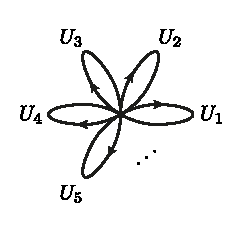
\includegraphics{petal2.pdf}
\end{center}
where the hamiltonian is given by
\begin{equation}
	H = \frac{g^2}{2 a} \sum_{j=1}^n \widehat{\ell}^2_j - \frac{2}{g^2 a} \sum_{j=1}^n \text{Re}(\tr(\widehat{u}_j\widehat{u}_{j+1}^\dag)).
\end{equation}
We introduce the following vector of hermitian operators
\begin{equation}
	[\widehat{\mathbf{n}}_j]_\alpha \equiv \frac12\tr((\tau^\alpha)^\dag \widehat{u}_j),
\end{equation}
in terms of which our hamiltonian becomes 
\begin{equation}
	H = \frac{g^2}{2 a} \sum_{j=1}^n \widehat{\ell}^2_j - \frac{4}{g^2 a} \sum_{j=1}^{n-1} \widehat{\mathbf{n}}_j\cdot \widehat{\mathbf{n}}_{j+1}.
\end{equation}
where we've exploited the identity
\begin{equation}
	\begin{split}
		\widehat{\mathbf{n}}\cdot \widehat{\mathbf{m}} &\equiv \sum_{\alpha = 0}^3 [\widehat{\mathbf{n}}]_\alpha [\widehat{\mathbf{m}}]_\alpha = \sum_{\alpha = 0}^3 \frac14\tr((\tau^\alpha)^\dag \widehat{u})\tr((\tau^\alpha)^\dag \widehat{v}^\dag) \equiv \frac12\sum_{\alpha = 0}^3 \tr((\tau^\alpha\otimes\tau^\alpha)^\dag \widehat{u}\otimes \widehat{v}) \\
		&=\frac12 \tr\left[ \left(|\tfrac12, -\tfrac12\rangle\langle \tfrac12, -\tfrac12| - |\tfrac12, -\tfrac12\rangle\langle -\tfrac12, \tfrac12| - |-\tfrac12, \tfrac12\rangle\langle \tfrac12, -\tfrac12| + |-\tfrac12, \tfrac12\rangle\langle -\tfrac12, \tfrac12|\right)\widehat{u}\otimes \widehat{v}\right] \\
		&= \frac12 [\widehat{u}]_{\tfrac12,\tfrac12}[\widehat{v}]_{-\tfrac12,-\tfrac12} - \frac12 [\widehat{u}]_{\tfrac12,-\tfrac12}[\widehat{v}]_{-\tfrac12,\tfrac12}-\frac12 [\widehat{u}]_{-\tfrac12,\tfrac12}[\widehat{v}]_{\tfrac12,-\tfrac12}+\frac12 [\widehat{u}]_{-\tfrac12,-\tfrac12}[\widehat{v}]_{\tfrac12,\tfrac12} \\
		&= \frac12 [\widehat{u}]_{\tfrac12,\tfrac12}[\widehat{v}^\dag]_{\tfrac12,\tfrac12} + \frac12 [\widehat{u}]_{\tfrac12,-\tfrac12}[\widehat{v}^\dag]_{-\tfrac12,\tfrac12}+\frac12 [\widehat{u}]_{-\tfrac12,\tfrac12}[\widehat{v}^\dag]_{\tfrac12,-\tfrac12}+\frac12 [\widehat{u}]_{-\tfrac12,-\tfrac12}[\widehat{v}^\dag]_{-\tfrac12,-\tfrac12} \\
		&= \frac12 \tr(\widehat{u}\widehat{v}^\dag). 
	\end{split}
\end{equation}

It is convenient to define the relative \emph{angle operator} $\widehat{\phi}_{jk}$ via
\begin{equation}
	\widehat{\phi}_{jk} \equiv \arccos\left(\frac12\widehat{\mathbf{n}}_j\cdot \widehat{\mathbf{n}}_{j+1}\right)
\end{equation}

We note that the commutation relations between the momenta and $\widehat{u}$:
\begin{equation}
	[\widehat{\ell}^\alpha, \widehat{u}_{jk}] = i[\tau^\alpha \widehat{u}]_{jk}
\end{equation}
imply that 
\begin{equation}
	[\widehat{\ell}^\alpha, \widehat{n}_\beta] = \left[\widehat{\ell}^\alpha, \frac{1}{2}\tr((\tau^\beta)^\dag \widehat{u})\right] = i\frac{1}{2}\tr((\tau^\beta)^\dag\tau^\alpha \widehat{u}) = -{\epsilon^{\alpha\beta}}_\gamma \widehat{n}_\gamma.
\end{equation}


We thus see that the Kogut-Susskind model compactified to a cylinder is equivalent to a $N=4$ rotor model on the line \cite{sachdev:2011a}.

Now we study the basic ground-state ansatz and its improvements for this simple model.

The basic ansatz corresponds to a sequence of states $|\Psi_m\rangle$, $m = 0, 1, \ldots$, which are given by successive quantum interpolations of the lattice strong-coupling state $|\Psi_0\rangle \equiv |\Omega_\infty\rangle$. Here we study the renormalisation of the hamiltonian $H$ under a quantum interpolation step. 

In the special case considered here a quantum interpolation step works as follows
\begin{equation}
	\begin{split}
		|\mathbf{U}\rangle \equiv \cdots |U_j\rangle |U_{j+1}\rangle \cdots &\mapsto \cdots |U_j\rangle |(U_{j+1} U_j^\dag)^{\frac12} U_j\rangle |U_{j+1}\rangle  |(U_{j+2} U_{j+1}^\dag)^{\frac12} U_{j+1}\rangle  \cdots \\
		&\equiv \textsl{C}\mathcal{U}|\mathbf{U}\rangle.
	\end{split}
\end{equation}
Suppose we have some initial state
\begin{equation}
	|\Psi\rangle \equiv \int d\mathbf{U}\, \psi(\mathbf{U}) |\mathbf{U}\rangle.
\end{equation}
We then interpolate the state to produce
\begin{equation}
	\textsl{C}\mathcal{U}|\Psi\rangle \equiv \int d\mathbf{U}\, \psi(\mathbf{U}) \textsl{C}\mathcal{U}|\mathbf{U}\rangle.
\end{equation}
The potential energy of the interpolated state is then given by the potential energy in the original state as follows
\begin{equation}
	\begin{split}
		\langle \Psi|\textsl{C}\mathcal{U}^\dag (\widehat{\mathbf{n}}_{2k}\cdot \widehat{\mathbf{n}}_{2k+1} )\textsl{C}\mathcal{U}|\Psi\rangle &= \int d\mathbf{U}d\mathbf{U}'\, \overline{\psi(\mathbf{U})}\psi(\mathbf{U})  \langle \mathbf{U}'|\textsl{C}\mathcal{U}^\dag (\widehat{\mathbf{n}}_{2k}\cdot \widehat{\mathbf{n}}_{2k+1} )\textsl{C}\mathcal{U}|\mathbf{U}\rangle \\
		&= \frac12\int d\mathbf{U}d\mathbf{U}'\, \overline{\psi(\mathbf{U})}\psi(\mathbf{U})  \langle \mathbf{U}'|\textsl{C}\mathcal{U}^\dag ( \tr(\widehat{u}_{2k}\widehat{u}^\dag_{2k+1}) )\textsl{C}\mathcal{U}|\mathbf{U}\rangle \\
		&= \frac12\int d\mathbf{U}d\mathbf{U}'\,  \tr((U_{j} U_{j+1}^\dag)^{\frac12} )  \overline{\psi(\mathbf{U})}\psi(\mathbf{U})  \langle \mathbf{U}'|\textsl{C}\mathcal{U}^\dag \textsl{C}\mathcal{U}|\mathbf{U}\rangle \\
		&= \frac12\int d\mathbf{U}d\mathbf{U}'\,  \tr((U_{j} U_{j+1}^\dag)^{\frac12} )  \overline{\psi(\mathbf{U})}\psi(\mathbf{U})  \langle \mathbf{U}'|\mathbf{U}\rangle \\
		&= \frac12\int d\mathbf{U}d\mathbf{U}'\,    \overline{\psi(\mathbf{U})}\psi(\mathbf{U})  \langle \mathbf{U}'|\tr(\widehat{u}_{k}\widehat{u}^\dag_{k+1}))^{\frac12} )|\mathbf{U}\rangle
	\end{split}
\end{equation}

\subsection{The ladder}
Lattice gauge theory on a ladder
\begin{center}
	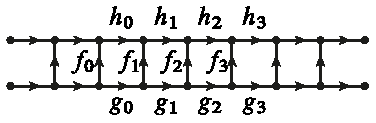
\includegraphics{ymladder.pdf}
\end{center}
is one of the first nontrivial gauge theories. Here we exploit the plaquette subdivision interpolation method to build a tensor network whose infrared limit is strongly coupled and whose ultraviolet limit is asymptotically free.

The key step is the isometry
\begin{multline}
	V_j = \int df_{j}df_{j+2}dg_j dg_{j+1}dh_j dh_{j+1} \\ |f_{j}f_{j+2}g_j g_{j+1}h_j h_{j+1}\rangle \langle f_{j}f_{j+2}g_j g_{j+1}h_j h_{j+1}| \otimes |W(f_{j},f_{j+2},g_j, g_{j+1},h_j, h_{j+1})\rangle,
\end{multline}
where $W$ is the interpolation of the two halves of the plaquette:
\begin{equation}
	W(f_{j},f_{j+2},g_j, g_{j+1},h_j, h_{j+1}) =  \frac{g_j^\dag f_j  h_j + g_{j+1}f_{j+2}h_{j+1}^\dag}{\sqrt{2 + \text{Re}(\tr(h_j^\dag f_j^\dag g_j g_{j+1}f_{j+2}h_{j+1}^\dag ))}}.
\end{equation}
Consider the action of the isometry $V_j$ on a plaquette operator $\text{Re}(\tr(\widehat{u}_{\square}))$, for 
\begin{equation}
	\text{Re}(\tr(\widehat{u}_{\square})) = \text{Re}(\tr(\widehat{u}^\dag(v_j,v_{j+1}) \widehat{u}(v_j,w_{j})\widehat{u}(w_j,w_{j+1})\widehat{u}(w_{j+1},w_{j+2})\widehat{u}^\dag(v_{j+2},w_{j+2}) \widehat{u}^\dag(v_{j+1},v_{j+2}))) 
\end{equation}
\begin{equation}
	V_j^\dag \text{Re}(\tr(\widehat{u}_{\square})) V_j = 
\end{equation}

\section{An ansatz for the ground-state wavefunction of pure lattice gauge theory}

\section{Summary and conclusions}

\bibliography{tnslgt}{}

\newpage
\appendix
\section{Group theory}

\subsection{Parametrisation}
In this subsection we detail the parametrisations of $\su2$ we exploit in the paper. The group $\su2$ consists of the set of all $2\times 2$ unimodular unitary matrices:
\begin{equation}
	U = \begin{pmatrix} \alpha & -\overline{\beta} \\ \beta & \overline{\alpha}\end{pmatrix}, \quad |\alpha|^2 + |\beta|^2 = 1.
\end{equation}
Thus, every element $U\in \su2$ is uniquely determined by two complex numbers $\alpha$ and $\beta$ subject to the constraint $|\alpha|^2 + |\beta|^2 = 1$. These are, in turn, given by three real parameters, e.g., $|\alpha|$, $\arg(\alpha)$, and $\arg(\beta)$. But if $\alpha\beta \not=1$, there is a more convenient parametrisation in terms of the \emph{Euler angles} $\varphi, \theta, \psi$ defined by
\begin{equation}
	|\alpha| = \cos\left(\frac{\theta}{2}\right), \quad \arg(\alpha) = \frac{\varphi +\psi}{2}, \quad \text{and} \quad  \arg(\beta) = \frac{\psi-\varphi + \pi}{2}.
\end{equation}
We demand that
\begin{equation}
	0\le \varphi < 2\pi, \quad 0\le \theta < \pi, \quad \text{and} \quad -2\pi \le \psi < 2\pi.
\end{equation}
In this case the correspondence $(\alpha, \beta) \leftrightarrow (\varphi, \theta, \psi)$, where $\alpha\beta \not=1$ and $|\alpha|^2 + |\beta|^2 = 1$ is one to one. An element $u\in \su2$ is given in terms of the Euler angles as
\begin{equation}
	U(\varphi, \theta, \psi) = \begin{pmatrix} \cos\left(\frac{\theta}{2}\right)e^{i(\varphi+\psi)/2} &  i\sin\left(\frac{\theta}{2}\right)e^{i(\varphi-\psi)/2}\\ i\sin\left(\frac{\theta}{2}\right)e^{-i(\varphi-\psi)/2} & \cos\left(\frac{\theta}{2}\right)e^{-i(\varphi+\psi)/2}\end{pmatrix}.
\end{equation}
We have the following factorisation 
\begin{equation}
	\begin{split}
	U(\varphi, \theta, \psi) &= U(\varphi, 0, 0)U(0, \theta, 0)U(0, 0, \psi) \equiv \\
	&= \begin{pmatrix}e^{i\varphi/2} & 0 \\ 0 & e^{-i\varphi/2}\end{pmatrix}\begin{pmatrix} \cos\left(\frac{\theta}{2}\right)& i\sin\left(\frac{\theta}{2}\right)\\ i\sin\left(\frac{\theta}{2}\right) & \cos\left(\frac{\theta}{2}\right)\end{pmatrix}\begin{pmatrix}e^{i\psi/2} & 0 \\ 0 & e^{-i\psi/2}\end{pmatrix}.
	\end{split}
\end{equation}



\subsection{Lie algebra of the group $\textsl{SU}(2)$}
We choose the three one-parameter subgroups $\Omega_1$, $\Omega_2$, and $\Omega_3$ of \su2 consisting of
\begin{equation}
	\omega_1(t) = u(0,t,0), \quad \omega_2(t) = \begin{pmatrix} \cos\left(\frac{t}{2}\right)& -\sin\left(\frac{t}{2}\right)\\ \sin\left(\frac{t}{2}\right) & \cos\left(\frac{t}{2}\right)\end{pmatrix}, \quad \text{and} \quad \omega_3(t) = u(t, 0, 0),
\end{equation}
respectively. The tangent matrices to these subgroups at the identity are
\begin{equation}
	a_1 = \frac{i}{2}\begin{pmatrix} 0& 1\\ 1 & 0\end{pmatrix}, \quad a_2 = \frac{1}{2}\begin{pmatrix} 0& -1\\ 1 & 0\end{pmatrix}, \quad \text{and} \quad a_3 = \frac{i}{2}\begin{pmatrix} 1 & 0\\ 0 & -1\end{pmatrix},
\end{equation}
respectively. These matrices are linearly independent and give a basis for the Lie algebra $\lasu2$ of \su2:
\begin{equation}
	[a_1, a_2] = a_3, \quad [a_2, a_3] = a_1, \quad \text{and} \quad [a_3, a_1] = a_2.
\end{equation}
The \emph{Casimir} operator for $\lasu2$ is given by
\begin{equation}
	c = a_1^2 + a_2^2 +a_3^2.
\end{equation}

\subsection{Identities}
Here we summarise a collection of useful identities for the group $\su2$ and the lie algebra $\lasu2$.

The first identity we review is the action of $\su2$ on the lie algebra: let $U\in\su2$, then
\begin{equation}
	U^\dag \sigma^j U  = \sum_{k=1}^3[\mathbf{O}]_{jk}\sigma^k,
\end{equation}
where
\begin{equation}
	\mathbf{O} = \begin{pmatrix} \Real(\alpha^2 - \beta^2) &  \Imag(\alpha^2 - \beta^2) & 2\Real(\alpha\overline{\beta}) \\ -\Imag(\alpha^2 + \beta^2) & \Real(\alpha^2+\beta^2) & -2\Imag(\alpha\overline{\beta}) \\ -2\Real(\alpha\beta) &  -2\Imag(\alpha\beta) & |\alpha|^2-|\beta|^2\end{pmatrix}.
\end{equation}
The matrix $\mathbf{O}$ is an orthogonal matrix.

From this equation we see that the action of $U$ on a traceless hermitian operators $X = \mathbf{x}\cdot\boldsymbol{\sigma} \equiv x_1\sigma^1 + x_2\sigma^2 +x_3\sigma^3$ is given by
\begin{equation}
	U^\dag  (\mathbf{x}\cdot\boldsymbol{\sigma}) U  = \sum_{j,k=1}^3 x_j [\mathbf{O}]_{jk}\sigma^k = (\mathbf{x}\mathbf{O})\cdot.\boldsymbol{\sigma}
\end{equation}

The next result concerns the product of two traceless hermitian operators $X = \mathbf{x}\cdot\boldsymbol{\sigma} \equiv x_1\sigma^1 + x_2\sigma^2 +x_3\sigma^3$ and $Y = \mathbf{y}\cdot \boldsymbol{\sigma}$. We find
\begin{equation}
	XY = (\mathbf{x}\cdot\boldsymbol{\sigma})(\mathbf{y}\cdot\boldsymbol{\sigma}) = (\mathbf{x}\cdot \mathbf{y})\mathbb{I} + i (\mathbf{x}\times \mathbf{y})\cdot \boldsymbol{\sigma}.
\end{equation}

Now consider the diagonalisation of $U\in \su2$. To tackle this problem we first study how to diagonalise traceless hermitian operators of the form $X = \mathbf{x}\cdot\boldsymbol{\sigma}$ with $\|\mathbf{x}\|=1$. This problem is equivalent to finding the rotation matrix $\mathbf{O}\in \o3$ which rotates the unit vector $\mathbf{x}$ to $\widehat{k} = (0,0,1)$. Here we directly solve the problem as follows. The normalised eigenvectors of $X$ are 
\begin{equation}
	v_{+1} \equiv \sqrt{\frac{1+x_3}{2}}\begin{pmatrix} 1 \\ \frac{x_1+ix_2}{1+x_3}\end{pmatrix}, \quad \text{and}\quad v_{-1} \equiv \sqrt{\frac{1+x_3}{2}}\begin{pmatrix}  \frac{-x_1+ix_2}{1+x_3} \\ 1\end{pmatrix},
\end{equation}
corresponding to eigenvalues $\lambda_+=+1$ and $\lambda_- = -1$, respectively. Using $v_\pm$ we construct the matrix $V\in\su2$
\begin{equation}
	V = \sqrt{\frac{1+x_3}{2}}\begin{pmatrix} 1 & \frac{-x_1+ix_2}{1+x_3}\\ \frac{x_1+ix_2}{1+x_3} & 1\end{pmatrix},
\end{equation}
diagonalising $X$ as $V^\dag X V = \sigma^z$. It is convenient to find the exponential representation of $V$:
\begin{equation}
	V = e^{i \omega\mathbf{v}\cdot\boldsymbol{\sigma}},
\end{equation} 
with $\omega = \cos^{-1}\left(\sqrt{\frac{1+x_3}{2}}\right)$, and
\begin{equation}
	\mathbf{v} = \frac{1}{\sqrt{x_1^2 + x_2^2}} (x_2, -x_1, 0).
\end{equation}

The product of two elements $U$ and $V$ of $\su2$ may be expressed in the  exponential representation as
\begin{equation}
	\begin{split}
	UV &= (\cos(\alpha)\mathbb{I} + i\sin(\alpha)\mathbf{u}\cdot\boldsymbol{\sigma})(\cos(\beta)\mathbb{I} + i\sin(\beta)\mathbf{v}\cdot\boldsymbol{\sigma}) \\
	&= [\cos(\alpha)\cos(\beta) - \sin(\alpha)\sin(\beta) (\mathbf{u}\cdot\mathbf{v})] \mathbb{I} + \\& \quad\quad\quad i [\sin(\alpha)\cos(\beta)\mathbf{u} + \cos(\alpha)\sin(\beta)\mathbf{v} - \sin(\alpha)\sin(\beta) (\mathbf{u}\times \mathbf{v})]\cdot\boldsymbol{\sigma} \\ 
	&= \cos(\gamma) \mathbb{I} + i\sin(\gamma) \mathbf{w}\cdot\boldsymbol{\sigma},
	\end{split}
\end{equation}
where 
\begin{equation}
	\cos(\gamma) = \cos(\alpha)\cos(\beta) - \sin(\alpha)\sin(\beta) (\mathbf{u}\cdot\mathbf{v}),
\end{equation}
and
\begin{equation}
	\mathbf{w} = \frac{\sin(\alpha)\cos(\beta)\mathbf{u} + \cos(\alpha)\sin(\beta)\mathbf{v} - \sin(\alpha)\sin(\beta) (\mathbf{u}\times \mathbf{v})}{\sin(\gamma)}.
\end{equation}

\subsection{Invariant measure}
We write an arbitrary element $U$ of $\su2$ as 
\begin{equation}
	U = \sum_{\mu=0}^3 u_\mu \tau^\mu,
\end{equation}
where
\begin{equation}
	\tau^0 =\begin{pmatrix}1 & 0 \\ 0 & 1\end{pmatrix}, \quad \tau^1 = {i}\begin{pmatrix} 0& 1\\ 1 & 0\end{pmatrix}, \quad \tau^2 = i\begin{pmatrix} 0& -i\\ i & 0\end{pmatrix}, \quad \text{and} \quad \tau^3 = {i}\begin{pmatrix} 1 & 0\\ 0 & -1\end{pmatrix},
\end{equation}
respectively. Recall that
\begin{equation}
	(\tau^{\mu},\tau^{\nu}) = 2\delta^{\mu\nu}, 
\end{equation}
where $(A,B) \equiv \tr(A^\dag B)$ and the constraints of unitarity and $\det(U) = 1$ imply that
\begin{equation}
	\sum_{\alpha=0}^3 u_\alpha^2 = 1.
\end{equation}
We can write the invariant Haar measure naturally in terms of spherical polar coordinates
\begin{equation}
	\begin{split}
	u_0 &= \cos(\phi_1), \\
	u_1 &= \sin(\phi_1)\cos(\phi_2), \\
	u_2 &= \sin(\phi_1)\sin(\phi_2)\cos(\phi_3), \quad \text{and} \\
	u_3 &= \sin(\phi_1)\sin(\phi_2)\sin(\phi_3).
	\end{split}
\end{equation}
The invariant measure of the sphere $S^3$ naturally gives the Haar measure, the Haar integral of a function $f:S^3 \rightarrow \mathbb{C}$ is then
\begin{equation}
	\int f(U) \, dU \equiv \frac{1}{2\pi^2}\int_{0}^{\pi}\int_{0}^\pi  \int_{0}^{2\pi} f(\phi_1,\phi_2,\phi_3)\sin^2(\phi_1)\sin(\phi_2)\, d\phi_1 d\phi_2 d\phi_3.
\end{equation}
If $f$ is a class function then $f(\phi_1,\phi_2,\phi_3) = f(\phi_1)$ and we obtain
\begin{equation}
	\int f(U)\, dU = \frac{2}{\pi}\int_0^\pi f(\phi_1)\sin^2(\phi_1)\,d\phi_1.
\end{equation}
An important example that results from our interpolation scheme is the class function
\begin{equation}
	f(\phi_1) = \cos\left(\frac{\phi_1}{n}\right).
\end{equation}
In this case we find
\begin{equation}
	\begin{split}
		\int \tr(U^{\frac1n})\, dU &= \frac{4}{\pi}\int_0^\pi \cos\left(\frac{\phi_1}{n}\right)\sin^2(\phi_1)\,d\phi_1 \\ 
		&= \frac{1}{\pi}\left[2n\sin\left(\frac{\phi_1}{n}\right) - \frac{n}{2n+1}\sin\left(\left[2+\frac{1}{n}\right]\phi_1\right)- \frac{n}{2n-1}\sin\left(\left[2-\frac{1}{n}\right]\phi_1\right)\right]_0^\pi \\
		&= \frac{1}{\pi}\left[2n\sin\left(\frac{\pi}{n}\right) - \frac{n}{2n+1}\sin\left(\frac{\pi}{n}\right) + \frac{n}{2n-1}\sin\left(\frac{\pi}{n}\right)\right] \\
		&= \frac{1}{\pi} \frac{8n^3}{4n^2 -1} \sin\left(\frac{\pi}{n}\right).
		\end{split}
\end{equation}

The invariant measure on \su2 is of the form
\begin{equation}
	du = N \delta(|\alpha|^2 + |\beta|^2 - 1)d\alpha_1d\alpha_2d\beta_1\beta_2,
\end{equation}
where $\alpha = \alpha_1 + i\alpha_2$, $\beta = \beta_1 + i\beta_2$, and $N$ is a normalisation. In terms of the Euler angles the invariant integral on \su2
has the form
\begin{equation}
	\int f(u) \, du = \frac{1}{16\pi^2} \int_{-2\pi}^{2\pi} \int_0^\pi \int_0^{2\pi} f(\varphi, \theta, \psi) \sin(\theta)\, d\varphi d\theta d\psi.
\end{equation}

\subsection{Finite-dimensional irreducible representations of \su2}
\subsubsection{Representations on the space of homogeneous polynomials}
Let $\ell \in \frac12\mathbb{Z}^+$. We denote by $\mathfrak{h}_\ell$ the space of all homogeneous polynomials
\begin{equation}
	f(z_1, z_2) = \sum_{n=-\ell}^\ell f_n z_1^{\ell-n}z_2^{\ell+n}
\end{equation}
in two complex variables of degree $2\ell$. For every element $g = \left(\begin{smallmatrix}\alpha & \beta \\ \gamma &\delta\end{smallmatrix}\right) \in \gl2c$ we have the representation on $\mathfrak{h}_\ell$ given by
\begin{equation}
	(T_\ell(g)f)(z_1, z_2) = f(\alpha z_1 + \gamma z_2, \beta z_1 + \delta z_2).
\end{equation}
On the complex line $z_2 = 1$ every polynomial $f\in \mathfrak{h}_\ell$ is determined by a polynomial $F(z) = \sum_{n=-\ell}^\ell f_n z^{\ell-n}$ of degree $2\ell$ in one variable according to 
\begin{equation}
	f(z_1, z_2)  = z_2^{2\ell} F\left(\frac{z_1}{z_2}\right).
\end{equation}
The realisation of the operator $T_\ell(g)$ on the space of polynomials of degree $2\ell$ in one variable is given by
\begin{equation}
	(T_\ell(g)F)(z) = (\beta z + \delta)^{2\ell} F\left(\frac{\alpha z + \gamma}{\beta z + \delta}\right).
\end{equation}
This representation can also be realised on the space of trigonometric polynomials of degree $\ell$. To do this we associate with every polynomial $F(z) = \sum_{n=-\ell}^\ell f_n z^{\ell-n}$ a trigonometric polynomial
\begin{equation}
	\Phi(e^{i\varphi}) = e^{-i\ell\varphi}F(e^{i\varphi}) = \sum_{n=-\ell}^\ell f_n e^{in\varphi}.
\end{equation}
We thus obtain the representation 
\begin{equation}
	(T_\ell(g)\Phi)(e^{i\varphi}) = e^{-i\ell\varphi}(\alpha e^{i\varphi} + \gamma)^{\ell}(\beta e^{i\varphi} + \delta)^{\ell} \Phi\left(\frac{\alpha e^{i\varphi} + \gamma}{\beta e^{i\varphi} + \delta}\right).
\end{equation}

\subsubsection{Infinitesimal operators}
We find the infinitesimal operators representing $a_1$, $a_2$, and $a_3$ for the one-parameter subgroups $\Omega_1$, $\Omega_2$, and $\Omega_3$ of \su2 on the space of polynomials of degree $2\ell$ in one variable. We obtain
\begin{equation}
	A_1 = i\ell x + \frac{i}{2}(1-x^2)\frac{d}{dx}, \quad A_2 = -\ell x + \frac12(1+x^2) \frac{d}{dx}, \quad \text{and} \quad A_3 = i\left(x\frac{d}{dx} - \ell\right).
\end{equation}

\subsubsection{An alternative construction of the irreps of \su2}
In this section we describe a simple quantum-information inspired mnemonic to remember how to construct the irreps of \su2. To carry out this construction all we need to remember are the following objects. Consider $2\ell$ qubits, $\ell \in \frac12\mathbb{Z}^+$, with hilbert space $\mathcal{H}_\ell \cong \mathbb{C}^{2^{2\ell}}$, and construct the \emph{generalised $W$ states}:
\begin{equation}
	\begin{split}
		|W_{\ell}\rangle &\equiv |\uparrow\dots \uparrow\rangle \\
		|W_{\ell-1}\rangle &\equiv \frac{1}{\sqrt{2\ell }} \left(|\downarrow \uparrow\uparrow\dots \uparrow\rangle + |\uparrow\downarrow\uparrow\dots \uparrow\rangle + \cdots + |\uparrow\dots \uparrow\downarrow\rangle\right) \\
		|W_{\ell-2}\rangle &\equiv \frac{1}{\sqrt{\binom{2\ell }{2}}} \left(|\downarrow\downarrow\uparrow\dots \uparrow\rangle + |\downarrow\uparrow\downarrow\dots \uparrow\rangle + \cdots + |\uparrow\dots \uparrow\downarrow\downarrow\rangle\right)\\
		&\vdots \\
		|W_{j}\rangle &\equiv \frac{1}{\sqrt{\binom{2\ell }{\ell-j}}} \left(|\underbrace{\downarrow\cdots\downarrow}_{\text{$\ell-j$ }} \underbrace{\uparrow\cdots \uparrow}_{\text{$\ell+j$}}\rangle + \text{permutations}\right) \\
		&\vdots \\
		|W_{-\ell}\rangle &\equiv |\downarrow\downarrow\dots \downarrow\rangle. \\
	\end{split}
\end{equation}
The generalised $W$-state $|W_j\rangle$ is an equal superposition over all permutations of $j$ down arrows and $2\ell - j$ up arrows.  

Given these states and the simple fact that the $2\ell$-fold tensor product $U\otimes \cdots \otimes U$ maps the subspace of $\mathcal{H}_\ell$ to itself we construct the matrix elements of the irrep of \su2 labelled by $\ell$ via
\begin{equation}
	\tau_{jk}^\ell(U) \equiv \langle W_j| U\otimes \cdots \otimes U |W_k\rangle, \quad j,k = -\ell, -\ell+1, \ldots, \ell.
\end{equation}
We can now directly derive the orthonormality of the matrix elements $\tau_{jk}^\ell(U)$ according to the inner product induced by the haar measure. Write
\begin{equation}
		({\tau}^{\ell'}_{j'k'}, {\tau}^{\ell}_{jk}) \equiv \int dU\,\overline{\tau}^{\ell'}_{j'k'}(U){\tau}^{\ell}_{jk}(U) = \int dU\, \langle W_{k'}| \underbrace{U^\dag \otimes \cdots \otimes U^\dag}_{\text{$2\ell'$ times}}  |W_{j'}\rangle \langle W_j| \underbrace{U\otimes \cdots \otimes U}_{\text{$2\ell$ times}} |W_k\rangle.
\end{equation}
From this expression we immediately deduce that for the RHS to be nonzero we need $\ell' = \ell$ (just use the left invariance of the haar measure). To deduce the rest of the result we simply exploit the left invariance of the haar measure to change variables to $V = \Phi U$, where $\Phi = e^{i\phi \sigma^z}$:
\begin{multline}
		({\tau}^{\ell'}_{j'k'}, {\tau}^{\ell}_{jk}) = \int dV\, \langle W_{k'}| \underbrace{V^\dag \otimes \cdots \otimes V^\dag}_{\text{$2\ell'$ times}}  (\Phi^\dag\otimes \cdots \otimes \Phi^\dag)|W_{j'}\rangle \langle W_j|(\Phi\otimes \cdots \otimes \Phi) \underbrace{V\otimes \cdots \otimes V}_{\text{$2\ell$ times}} |W_k\rangle \\ = e^{-2i j'\phi }e^{2ij\phi} ({\tau}^{\ell'}_{j'k'}, {\tau}^{\ell}_{jk}) = e^{2i\phi (j-j')} ({\tau}^{\ell'}_{j'k'}, {\tau}^{\ell}_{jk}).
\end{multline}
Since this is true for all $\phi \in [0, \pi)$ we find that $j=j'$ in order for the inner product to be nonzero.
Similarly, we deduce that
\begin{equation}
	({\tau}^{\ell'}_{j'k'}, {\tau}^{\ell}_{jk}) = e^{2i\phi (k'-k)} ({\tau}^{\ell'}_{j'k'}, {\tau}^{\ell}_{jk}),
\end{equation}
so that we require $k = k'$ for the inner product to be nonzero. Finally, we exploit the completeness relation $\mathbb{I} = \sum_{j} |W_j\rangle \langle W_j|$ on the subspace spanned by the $W$ states to deduce that
\begin{equation}
	\sum_{j,k} ({\tau}^{\ell}_{jk}, {\tau}^{\ell}_{jk}) = 2\ell+1,
\end{equation} 
from which we readily deduce the value $1/(2\ell + 1)$ for the inner product $({\tau}^{\ell}_{jk}, {\tau}^{\ell}_{jk})$.

\subsection{Clebsch-Gordon coefficients}
We can use the representation described in the previous subsection to easily determine the Clebsch-Gordon coefficients for the addition of a single spin-$\frac12$ irrep. 

Suppose we want to decompose the product of irreps
\begin{equation}
	\tau_{\alpha\beta}^{\frac12}(U)\tau_{jk}^{\ell}(U)
\end{equation}
into a direct sum of irreps. We can achieve this by exploiting the ideas of the previous subsection. First write
\begin{equation}
	\begin{split}
		\tau_{\alpha\beta}^{\frac12}(U)\tau_{jk}^{\ell}(U) &\equiv \langle \alpha|U|\beta\rangle \langle W_j| \underbrace{U\otimes \cdots \otimes U}_{\text{$2\ell$ times}} |W_k\rangle \\
		&= \langle\alpha| \langle W_j| \underbrace{U\otimes U\otimes \cdots \otimes U}_{\text{$2\ell + 1$ times}} |\beta\rangle|W_k\rangle.
	\end{split}
\end{equation}
Write $P_{\ell}$ for the projection onto the subspace spanned by the $W$ states of $2\ell$ qubits. We know that $P_{\ell+\frac12} \subset \mathbb{I}_{\frac12}\otimes P_{\ell}$; indeed, we know that, under the action of $\underbrace{U\otimes U\otimes \cdots \otimes U}_{\text{$2\ell + 1$ times}}$ the projection $\mathbb{I}_{\frac12}\otimes P_{\ell}$ decomposes as
\begin{equation}
	\mathbb{I}_{\frac12}\otimes P_{\ell} = P_{\ell+\frac12} \oplus P_{\ell-\frac12}.
\end{equation}
Our task is to work out the unitary operation realising this decomposition. This is actually very easy: we know that the projection $P_{\ell+\frac12}$ onto the space spanned by the generalised $W$ states on $2\ell+1$ qubits is completely contained within $\mathbb{I}_{\frac12}\otimes P_{\ell}$, i.e.,
\begin{equation}
	P_{\ell+\frac12} \le \mathbb{I}_{\frac12}\otimes P_{\ell}
\end{equation}
in the positive semidefinite ordering. Hence we immediately obtain that
\begin{equation}
	P_{\ell-\frac12} \equiv (\mathbb{I} - P_{\ell+\frac12})\mathbb{I}_{\frac12}\otimes P_{\ell}.
\end{equation}
How do we find the unitary $U_{\text{CG}}$ rotating from the basis $|\alpha\rangle|W_j^{\ell}\rangle$ to the basis $\{|W_j^{\ell+\frac12}\rangle, |W_k^{\ell-\frac12}\rangle\,|\, j = -\ell-\frac12,\ldots, \ell+\frac12, k = -\ell+\frac12, \ldots, \ell - \frac12\rangle\}$? (Note that the vectors $|W_k^{\ell-\frac12}\rangle$ are not just simply the generalised $W$ states on $2\ell-1$ qubits; rather they are a basis for the subspace $(\mathbb{I} - P_{\ell+\frac12})\mathbb{I}_{\frac12}\otimes P_{\ell}$.) To build $U_{\text{CG}}$ we need the matrix elements
\begin{equation}
	c_{k,(\alpha,j)} = \langle W_k^{\ell+\frac12}|\alpha, W_j^{\ell}\rangle = \binom{2\ell+1}{\ell+\frac12-k}^{-\frac12}\binom{2\ell}{\ell-j}^{\frac12}, \quad k = j+\alpha,
\end{equation}
which simplifies to
\begin{equation}
	c_{k,(\alpha,j)} = \sqrt{\frac{\ell+2\alpha j + 1}{2\ell+1}}\delta_{k, j + \alpha},
\end{equation}
where $\alpha = \pm\frac12$. This gives us just over half of the matrix elements unitary transformation between the two bases. To complete our specification of $U_{CG}$ we need to find a basis of vectors for the subspace $(\mathbb{I} - P_{\ell+\frac12})\mathbb{I}_{\frac12}\otimes P_{\ell}$. We do this directly by observing that 
\begin{equation}
	d_{k',(\alpha,j)} = -2\alpha\sqrt{\frac{\ell-2\alpha j}{2\ell+1}}\delta_{k', j+\alpha}, \quad k' = -\ell+\frac12, \ldots, \ell-\frac12. 
\end{equation}
We hence obtain the unitary matrix
\begin{equation}
	U_{\text{CG}} = \sum_{k = -\ell-\frac12}^{\ell+\frac12} c_{k,(\alpha,j)} |k,\ell+\tfrac12\rangle \langle \alpha, j| + \sum_{k = -\ell+\frac12}^{\ell-\frac12} d_{k,(\alpha,j)}|k,\ell-\tfrac12\rangle\langle \alpha, j|.
\end{equation}

As an example consider the case $\ell = 1$; we find
\begin{equation}
	U_{\text{CG}} = 
	\begin{pmatrix}
		1 & 0 & 0 & 0 & 0 & 0   \\
		0 & \sqrt{\tfrac23} & 0 & \sqrt{\tfrac13} & 0 & 0  \\
		0 & 0 & \sqrt{\tfrac13} & 0 & \sqrt{\tfrac23} & 0  \\
		0 & 0 & 0 & 0 & 0 & 1  \\
		0 & \sqrt{\tfrac13} & 0 & -\sqrt{\tfrac23} & 0 & 0  \\
		0 & 0 & \sqrt{\tfrac23} & 0 & -\sqrt{\tfrac13} & 0  
	\end{pmatrix},
\end{equation}
where the rows are labelled by $[-\tfrac32, -\tfrac12, \tfrac12, \tfrac32, -\tfrac12, \tfrac12]$, and the columns by 

$[(-\tfrac12, -1), (-\tfrac12, 0), (-\tfrac12, 1), (\tfrac12, -1), (\tfrac12, 0), (\tfrac12, 1)]$.



\subsection{Diagonalising products of unitaries}\label{app:diagprod}
In this subsection we detail the calculations of the diagonalising matrix for a product $UV$ of two elements from $\su2$.

We first calculate the square root; there are three cases for $\alpha = 1,2, 3$. The first case is $\alpha = 1$:
\begin{equation}
	\begin{split}
		e^{i\epsilon \sigma^1}e^{i\phi \sigma^3} &= (\cos(\epsilon)\mathbb{I} + i\sin(\epsilon)\sigma^1)(\cos(\phi)\mathbb{I} + i\sin(\phi)\sigma^3) \\ 
		&= \cos(\epsilon)\cos(\phi)\mathbb{I} + i\sin(\epsilon)\cos(\phi)\sigma^1 - \sin(\epsilon)\sin(\phi)\sigma^1\sigma^3 + i\cos(\epsilon)\sin(\phi)\sigma^3 \\
		&= \cos(\epsilon)\cos(\phi)\mathbb{I} + i\sin(\epsilon)\cos(\phi)\sigma^1 + i\sin(\epsilon)\sin(\phi)\sigma^2 + i\cos(\epsilon)\sin(\phi)\sigma^3 \\
		&= \cos(\epsilon)\cos(\phi)\mathbb{I} + i\sqrt{\sin^2(\epsilon) + \cos^2(\epsilon)\sin^2(\phi)} \ \mathbf{x}(\epsilon)\cdot \boldsymbol{\sigma},
	\end{split}
\end{equation}
where
\begin{equation}
	\begin{split}
		x_1(\epsilon) &= \frac{\sin(\epsilon)\cos(\phi)}{\sqrt{\sin^2(\epsilon) + \cos^2(\epsilon)\sin^2(\phi)}}\\
		x_2(\epsilon) &= \frac{\sin(\epsilon)\sin(\phi)}{\sqrt{\sin^2(\epsilon) + \cos^2(\epsilon)\sin^2(\phi)}}\\
		x_3(\epsilon) &= \frac{\cos(\epsilon)\sin(\phi)}{\sqrt{\sin^2(\epsilon) + \cos^2(\epsilon)\sin^2(\phi)}}.
	\end{split}
\end{equation}
We now have enough information to calculate the square root $\sqrt{ e^{i\epsilon \sigma^\alpha}\Phi}$, we find
\begin{equation}
	\sqrt{ e^{i\epsilon \sigma^\alpha}\Phi} = W (\epsilon) \sqrt{D(\epsilon)}\ W^\dag(\epsilon),
\end{equation}
where
\begin{equation}
	\begin{split}
		D(\epsilon) &= e^{i\phi(\epsilon) \sigma^3}, \\
		W(\epsilon) &= \sqrt{\frac{1+x_3(\epsilon)}{2}}\begin{pmatrix} 1 & \frac{-x_1(\epsilon)+ix_2(\epsilon)}{1+x_3(\epsilon)}\\ \frac{x_1(\epsilon)+ix_2(\epsilon)}{1+x_3(\epsilon)} & 1\end{pmatrix}.
	\end{split}
\end{equation}
and
\begin{equation}
	\phi(\epsilon) = \cos^{-1}(\cos(\epsilon)\cos(\phi)).
\end{equation}
The $\epsilon=0$ derivative of the square root is now found by evaluating
\begin{equation}
	\frac{d}{d\epsilon} \left(W (\epsilon) \sqrt{D(\epsilon)}\ W^\dag(\epsilon)\right)\bigg|_{\epsilon =0},
\end{equation}
which, in turn, is found by calculating $D'(0)$ and $W'(0)$. Firstly, we have that 
\begin{equation}
	\frac{d}{d\epsilon} e^{i\frac{\phi(\epsilon)}{2}\sigma^3}\bigg|_{\epsilon=0} = 0.
\end{equation}
We then calculate the derivative of $W(\epsilon)$ by first evaluating
\begin{equation}
	\begin{split}
		\frac{dx_1(\epsilon)}{d\epsilon}\bigg|_{\epsilon=0} &= \frac{\cos(\phi)}{\sin(\phi)}\\
		\frac{dx_2(\epsilon)}{d\epsilon}\bigg|_{\epsilon=0} &= 1\\
		\frac{dx_3(\epsilon)}{d\epsilon}\bigg|_{\epsilon=0} &= 0.
	\end{split}
\end{equation}
These results can be used to conclude that
\begin{equation}
	\frac{d}{d\epsilon} W(\epsilon)\bigg|_{\epsilon=0} = \frac{1}{{2}}\begin{pmatrix} 0 & -\cot(\phi)+i\\ \cot(\phi)+i & 0\end{pmatrix}.
\end{equation}
Thus
\begin{multline}
	\frac{d}{d\epsilon} \left(W (\epsilon) \sqrt{D(\epsilon)}\ W^\dag(\epsilon)\right)\bigg|_{\epsilon =0} =\\ \frac{1}{{2}}\begin{pmatrix} 0 & -\cot(\phi)+i\\ \cot(\phi)+i & 0\end{pmatrix} e^{i\frac{\phi}{2} \sigma^3}
- \frac{1}{{2}}e^{i\frac{\phi}{2} \sigma^3}\begin{pmatrix} 0 & -\cot(\phi)+i\\ \cot(\phi)+i & 0\end{pmatrix}.
\end{multline}
Which reduces to
\begin{equation}
	\begin{split}
	\frac{d}{d\epsilon}\sqrt{e^{i\epsilon \sigma^1}\Phi}\bigg|_{\epsilon =0}\sqrt{\Phi^\dag} &= \begin{pmatrix} 0 & \sin(\frac{\phi}{2})(1+i\cot(\phi)) \\ -\sin(\frac{\phi}{2})(1-i\cot(\phi)) & 0\end{pmatrix} \sqrt{\Phi^\dag} \\ &=i(\sin(\tfrac{\phi}{2})\cot(\phi)\sigma^x + \sin(\tfrac{\phi}{2})\sigma^y)(\cos(\tfrac{\phi}{2})\mathbb{I} - i\sin(\tfrac{\phi}{2})\sigma^z)\\ &= i\sin(\tfrac{\phi}{2})\cos(\tfrac{\phi}{2})[(\cot(\phi) + \tan(\tfrac{\phi}{2})) \sigma^x + (1 - \tan(\tfrac{\phi}{2})\cot(\phi))\sigma^y ] \\
	&= i[ (\tfrac12\cos(\phi)+ \sin^2(\tfrac{\phi}{2}))\sigma^x + (\tfrac12 \sin(\phi) - \sin^2(\tfrac{\phi}{2})\cot(\phi))\sigma^y ] \\
	&= \frac{i}{2}\sigma^x + i\frac{1-\cos(\phi)}{2\sin(\phi)}\sigma^y.
	\end{split}
\end{equation}
Since 
\begin{equation}
	\sigma^y = e^{-i\frac{\pi}{4}\sigma^z}\sigma^xe^{i\frac{\pi}{4}\sigma^z}, \quad \text{and}\quad -\sigma^x = e^{-i\frac{\pi}{4}\sigma^z}\sigma^ye^{i\frac{\pi}{4}\sigma^z}
\end{equation}
we immediately obtain
\begin{equation}
	\frac{d}{d\epsilon}\sqrt{e^{i\epsilon \sigma^2}\Phi}\bigg|_{\epsilon =0}\sqrt{\Phi^\dag} = \frac{i}{2}\sigma^y - i\frac{1-\cos(\phi)}{2\sin(\phi)}\sigma^y.
\end{equation}
Finally, 
\begin{equation}
	\frac{d}{d\epsilon}\sqrt{e^{i\epsilon \sigma^3}\Phi}\bigg|_{\epsilon =0}\sqrt{\Phi^\dag} = \frac{i}{2}  \sigma^z.
\end{equation}
We summarise these three formula via
\begin{equation}
	\frac{d}{d\epsilon}\sqrt{e^{i\epsilon \sigma^j}\Phi}\sqrt{\Phi^\dag} \bigg|_{\epsilon =0} \equiv i\sum_{k=1}^3 [\phi]_{jk} \sigma^k,
\end{equation}
with 
\begin{equation}
	\phi = \begin{pmatrix}\frac12 & \frac{1-\cos(\phi)}{2\sin(\phi)} & 0 \\ -\frac{1-\cos(\phi)}{2\sin(\phi)} & \frac12 & 0 \\ 0 & 0 & \frac12\end{pmatrix}.
\end{equation}


The next step is to exploit the formula
\begin{equation}
	S^\dag \sigma^{j} S = \sum_{k = 1}^3 [\mathbf{O}]_{jk} \sigma^k,
\end{equation}
for $S \in \su2$. Using this formula we calculate
\begin{equation}
	\begin{split}
	\frac{d}{d\epsilon}\sqrt{e^{i\epsilon \sigma^j} VU^\dag}\sqrt{U^\dag V}\bigg|_{\epsilon =0} &= \frac{d}{d\epsilon}\sqrt{e^{i\epsilon \sigma^j} S \Phi S^\dag}\sqrt{S \Phi^\dag S^\dag}\bigg|_{\epsilon =0} \\
	&= S\left[\frac{d}{d\epsilon}\sqrt{e^{i\epsilon S^\dag \sigma^j S}  \Phi }\sqrt{ \Phi^\dag }\right]\bigg|_{\epsilon =0} S^\dag \\
	&= i \sum_{k=1}^3 [\mathbf{O} \phi ]_{jk}  S\sigma^k S^\dag \\
	&= i \sum_{k=1}^3 [\mathbf{O} \phi \mathbf{O}^T]_{jk}  \sigma^k, \\
	\end{split}
\end{equation}
where $S$ is the unitary operator diagonalising $VU^\dag$ and $\mathbf{O}$ is the orthogonal matrix corresponding to $S$.

The transformation of $\widehat{\ell}^j_L$ is given by
\begin{multline}
	\mathbb{I}\otimes \widehat{\ell}_L^{j}\otimes \mathbb{I}  -i\int dUdV \, |U\rangle\langle U| \otimes  |V\rangle\langle V| \otimes \frac{d}{d\epsilon} R_{\mathbf{I}(U,e^{i\epsilon \sigma^j}V) \mathbf{I}^\dag(U,V)}\bigg|_{\epsilon = 0} = \\
	\mathbb{I}\otimes \widehat{\ell}_L^{j}\otimes \mathbb{I} + \sum_{k=1}^3 \int dUdV \, [\mathbf{O} \phi \mathbf{O}^T]_{jk} |U\rangle\langle U| \otimes  |V\rangle\langle V| \otimes  \widehat{\ell}^k.
\end{multline}

\section{A detailed look at the quantum interpolation algorithm}
Here we detail the steps of the quantum interpolation algorithm. We work with a two-dimensional lattice. We label the connection variables on the edges pointing in the $\widehat{x}$ direction as $U_\mathbf{x}$, where $\mathbf{x}\in L$ is the source vertex and, correspondingly, the connection variables pointing in the $\widehat{y}$ direction as $V_\mathbf{x}$. The collection of all the $U_\mathbf{x}$ connection variables is written $\mathcal{U} \equiv (\cdots, U_\mathbf{x}, \cdots)$ and the $V_\mathbf{x}$ connection variables is written $\mathcal{V} \equiv (\cdots, V_\mathbf{x}, \cdots)$.


We begin by assuming that our lattice is in an arbitrary gauge invariant state:
\begin{equation}	
	|\Psi\rangle = \int d\mathcal{U}d\mathcal{V} \, \Psi(\mathcal{U},\mathcal{V}) |\mathcal{U},\mathcal{V}\rangle.
\end{equation}

The quantum interpolation algorithm proceeds in three major steps. The first step is to subdivide all the edges, i.e., we take each connection $U_\mathbf{x}$ and replace it with two connection variables: $U_\mathbf{x} X_\mathbf{x}$, with basepoint $\mathbf{x}$, and $X^\dag_{\mathbf{x}+\frac{a}{2}\hat{1}}$, with basepoint $\mathbf{x}+\frac{a}{2}\widehat{1}$ and integrate over $X_{\mathbf{x}} = X_{\mathbf{x}+\frac{a}{2}\hat{1}}$. Similarly, we replace $V_{\mathbf{x}}$ with two connection variables: $V_\mathbf{x} Y_\mathbf{x}$, with basepoint $\mathbf{x}$, and $Y^\dag_{\mathbf{x}+\frac{a}{2}\hat{2}}$, with basepoint $\mathbf{x}+\frac{a}{2}\hat{2}$). We end up with the state
\begin{equation}	
	|\Psi_1\rangle = \int d\mathcal{W}_1\, \Psi(\mathcal{U},\mathcal{V}) \left(\bigotimes_{\mathbf{x}\in L} |U_\mathbf{x} X_\mathbf{x}\rangle|X^\dag_{\mathbf{x}+\frac{a}{2}\hat{1}}\rangle|V_\mathbf{x} Y_\mathbf{x}\rangle|Y^\dag_{\mathbf{x}+\frac{a}{2}\hat{2}}\rangle \right),
\end{equation}
where 
\begin{equation}
d\mathcal{W}_1 \equiv  \bigotimes_{\mathbf{x}\in L} \delta(X_\mathbf{x}-X_{\mathbf{x}+\frac{a}{2}\hat{1}})\delta(Y_\mathbf{x} -Y_{\mathbf{x}+\frac{a}{2}\hat{2}}) dU_{\mathbf{x}} dV_{\mathbf{x}} dX_\mathbf{x} dX_{\mathbf{x}+\frac{a}{2}\hat{1}}dY_\mathbf{x} dY_{\mathbf{x}+\frac{a}{2}\hat{2}}.
\end{equation}
The next step is to introduce the ancillary states $\psi$, two per added lattice point $\mathbf{x}+\frac{a}{2}\widehat{1}$ and $\mathbf{x}+\frac{a}{2}\widehat{2}$:
\begin{multline}	
	|\Psi_2\rangle = \int  d\mathcal{W}_2 \, \Psi(\mathcal{U},\mathcal{V}) \bigotimes_{\mathbf{x}\in L}\Bigl( \psi(U_{\mathbf{x}+\frac{a}{2}\hat{2}}')\psi(U_{\mathbf{x}+{a}\hat{1}+\frac{a}{2}\hat{2}}')\psi(V_{\mathbf{x}+\frac{a}{2}\hat{1}}')\psi(V_{\mathbf{x}+\frac{a}{2}\hat{1}+{a}\hat{2}}') \times\\ 
	|U_\mathbf{x} X_\mathbf{x}\rangle|X^\dag_{\mathbf{x}+\frac{a}{2}\hat{1}}\rangle |U_{\mathbf{x}+\frac{a}{2}\hat{2}}'\rangle|U_{\mathbf{x}+{a}\hat{1}+\frac{a}{2}\hat{2}}'\rangle|V_\mathbf{x} Y_\mathbf{x}\rangle|Y^\dag_{\mathbf{x}+\frac{a}{2}\hat{2}}\rangle|V_{\mathbf{x}+\frac{a}{2}\hat{1}}'\rangle |V_{\mathbf{x}+\frac{a}{2}\hat{1}+{a}\hat{2}}'\rangle\Bigr),
\end{multline}
where $d\mathcal{W}_2 \equiv  d\mathcal{U}'d\mathcal{V}'d\mathcal{W}_1$.
The third and final step is to parallel transport the ends of the added links to the centres of the original plaquettes. To this end we first construct the auxiliary variables 
\begin{align}
	C_{(\mathbf{x}+\frac{a}{2}\hat{1}, \mathbf{x}+\frac{a}{2}\hat{2})} &\equiv X_{\mathbf{x}}^\dag U^\dag_{\mathbf{x}}V_\mathbf{x} Y_\mathbf{x} \\
	C_{(\mathbf{x}+\frac{a}{2}\hat{2}, \mathbf{x}+a\hat{2}+\frac{a}{2}\hat{1})} &\equiv Y_{\mathbf{x}+\frac{a}{2}\hat{2}}^\dag  U_{\mathbf{x}+a\hat{2}}X_{\mathbf{x} + a\hat{2}} \\
	C_{(\mathbf{x}+a\hat{2}+\frac{a}{2}\hat{1}, \mathbf{x}+a\hat{1}+\frac{a}{2}\hat{2})} &\equiv X_{\mathbf{x} + \frac{a}{2}\hat{1}+a\hat{2}}^\dag Y_{\mathbf{x}+a\hat{1}+\frac{a}{2}\hat{2}} \\
	C_{(\mathbf{x}+a\hat{1}+\frac{a}{2}\hat{2}, \mathbf{x}+\frac{a}{2}\hat{1})} &\equiv Y^\dag_{\mathbf{x}+a\hat{1}} V^\dag_{\mathbf{x}+a\hat{1}} X_{\mathbf{x}+\frac{a}{2}\hat{1}}.
\end{align}
We also construct the \emph{flux} through the plaquette based at $\mathbf{x}$:
\begin{equation}
	\Phi_\mathbf{x} = \eta^\dag_{\mathbf{x}} X_{\mathbf{x}+\frac{a}{2}\hat{1}}^\dag V_{\mathbf{x}+a\hat{1}} U_{\mathbf{x}+a\hat{2}}^\dag V_\mathbf{x}^\dag U_{\mathbf{x}}X_{\mathbf{x}}\eta_{\mathbf{x}},
\end{equation} 
where $\eta^\dag_{\mathbf{x}}$ is the matrix diagonalising $X_{\mathbf{x}+\frac{a}{2}\hat{1}}^\dag V_{\mathbf{x}+a\hat{1}} U_{\mathbf{x}+a\hat{2}}^\dag V_\mathbf{x}^\dag U_{\mathbf{x}}X_{\mathbf{x}}$.

Using the $C$ operators we then find the interpolating parallel transporters:
\begin{align}
	A_{(\mathbf{x}+\frac{a}{2}\hat{1}+\frac{a}{2}\hat{2}, \mathbf{x}+\frac{a}{2}\hat{2})} &\equiv \eta^\dag_{\mathbf{x}} X_{\mathbf{x}}^\dag U^\dag_{\mathbf{x}}V_\mathbf{x} Y_\mathbf{x} \\
	A_{(\mathbf{x}+\frac{a}{2}\hat{1}+\frac{a}{2}\hat{2}, \mathbf{x}+\frac{a}{2}\hat{1}+{a}\hat{2})} &\equiv \Phi_{\mathbf{x}}^{\frac14}\eta^\dag_{\mathbf{x}} X_{\mathbf{x}}^\dag U^\dag_{\mathbf{x}}V_\mathbf{x} U_{\mathbf{x}+a\hat{2}}X_{\mathbf{x} + a\hat{2}} \\
	A_{(\mathbf{x}+\frac{a}{2}\hat{1}+\frac{a}{2}\hat{2}, \mathbf{x}+{a}\hat{1}+\frac{a}{2}\hat{2})} &\equiv \Phi_{\mathbf{x}}^{\frac12}\eta^\dag_{\mathbf{x}} X_{\mathbf{x}}^\dag U^\dag_{\mathbf{x}}V_\mathbf{x} U_{\mathbf{x}+a\hat{2}} Y_{\mathbf{x}+a\hat{1}+\frac{a}{2}\hat{2}} \\
	A_{(\mathbf{x}+\frac{a}{2}\hat{1}+\frac{a}{2}\hat{2}, \mathbf{x}+\frac{a}{2}\hat{1})} &\equiv \Phi_{\mathbf{x}}^{\frac34}\eta^\dag_{\mathbf{x}} X_{\mathbf{x}}^\dag U^\dag_{\mathbf{x}}V_\mathbf{x}  U_{\mathbf{x}+a\hat{2}} V^\dag_{\mathbf{x}+a\hat{1}} X_{\mathbf{x}+\frac{a}{2}\hat{1}}.
\end{align}

Finally, we use the $A$s to parallel transport the new connection variables into the centres of the plaquettes:
\begin{multline}	
	|\Psi_3\rangle = \int  d\mathcal{W}_2 \, \Psi(\mathcal{U},\mathcal{V}) \bigotimes_{\mathbf{x}\in L}\Bigl( \psi(U_{\mathbf{x}+\frac{a}{2}\hat{2}}')\psi(U_{\mathbf{x}+{a}\hat{1}+\frac{a}{2}\hat{2}}')\psi(V_{\mathbf{x}+\frac{a}{2}\hat{1}}')\psi(V_{\mathbf{x}+\frac{a}{2}\hat{1}+{a}\hat{2}}') \times\\ 
	|U_\mathbf{x} X_\mathbf{x}\rangle|X^\dag_{\mathbf{x}+\frac{a}{2}\hat{1}}\rangle |U_{\mathbf{x}+\frac{a}{2}\hat{2}}' A_{(\mathbf{x}+\frac{a}{2}\hat{1}+\frac{a}{2}\hat{2}, \mathbf{x}+\frac{a}{2}\hat{2})}^\dag   \rangle|A_{(\mathbf{x}+\frac{a}{2}\hat{1}+\frac{a}{2}\hat{2}, \mathbf{x}+{a}\hat{1}+\frac{a}{2}\hat{2})}U_{\mathbf{x}+{a}\hat{1}+\frac{a}{2}\hat{2}}'\rangle \times \\ 
	|V_\mathbf{x} Y_\mathbf{x}\rangle|Y^\dag_{\mathbf{x}+\frac{a}{2}\hat{2}}\rangle|V_{\mathbf{x}+\frac{a}{2}\hat{1}}'A_{(\mathbf{x}+\frac{a}{2}\hat{1}+\frac{a}{2}\hat{2}, \mathbf{x}+\frac{a}{2}\hat{1})}^\dag\rangle |A_{(\mathbf{x}+\frac{a}{2}\hat{1}+\frac{a}{2}\hat{2}, \mathbf{x}+\frac{a}{2}\hat{1}+{a}\hat{2})}V_{\mathbf{x}+\frac{a}{2}\hat{1}+{a}\hat{2}}'\rangle \Bigr).
\end{multline}
We can now deduce the expectation value of a plaquette operator on the refined interpolated lattice in terms of its original expectation value. Consider the observable $\tr(\widehat{v}_{\mathbf{z}}\widehat{u}_{\mathbf{z}+\frac{a}{2}\hat{2}}\widehat{v}^\dag_{\mathbf{z}+\frac{a}{2}\hat{1}}\widehat{u}_{\mathbf{z}}^\dag)$, which is the curvature around the subplaquette with base point $\mathbf{z}$. It acts as a multiplication operator in the position basis, and on $|\Psi_3\rangle$ this is straightforward to calculate:
\begin{multline}	
	\tr(\widehat{v}_{\mathbf{z}}\widehat{u}_{\mathbf{z}+\frac{a}{2}\hat{2}}\widehat{v}^\dag_{\mathbf{z}+\frac{a}{2}\hat{1}}\widehat{u}_{\mathbf{z}}^\dag)|\Psi_3\rangle = \int  d\mathcal{W}_2 \, \Psi(\mathcal{U},\mathcal{V}) \times \\\tr(V_\mathbf{z} Y_\mathbf{z}U_{\mathbf{z}+\frac{a}{2}\hat{2}}' A_{(\mathbf{z}+\frac{a}{2}\hat{1}+\frac{a}{2}\hat{2}, \mathbf{z}+\frac{a}{2}\hat{2})}^\dag A_{(\mathbf{z}+\frac{a}{2}\hat{1}+\frac{a}{2}\hat{2}, \mathbf{z}+\frac{a}{2}\hat{1})}{V'}^\dag_{\mathbf{z}+\frac{a}{2}\hat{1}} X^\dag_\mathbf{z} U^\dag_\mathbf{z} )\\ \bigotimes_{\mathbf{x}\in L}\Bigl( \psi(U_{\mathbf{x}+\frac{a}{2}\hat{2}}')\psi(U_{\mathbf{x}+{a}\hat{1}+\frac{a}{2}\hat{2}}')\psi(V_{\mathbf{x}+\frac{a}{2}\hat{1}}')\psi(V_{\mathbf{x}+\frac{a}{2}\hat{1}+{a}\hat{2}}') \times\\ 
	|U_\mathbf{x} X_\mathbf{x}\rangle|X^\dag_{\mathbf{x}+\frac{a}{2}\hat{1}}\rangle |U_{\mathbf{x}+\frac{a}{2}\hat{2}}' A_{(\mathbf{x}+\frac{a}{2}\hat{1}+\frac{a}{2}\hat{2}, \mathbf{x}+\frac{a}{2}\hat{2})}^\dag   \rangle|A_{(\mathbf{x}+\frac{a}{2}\hat{1}+\frac{a}{2}\hat{2}, \mathbf{x}+{a}\hat{1}+\frac{a}{2}\hat{2})}U_{\mathbf{x}+{a}\hat{1}+\frac{a}{2}\hat{2}}'\rangle \times \\ 
	|V_\mathbf{x} Y_\mathbf{x}\rangle|Y^\dag_{\mathbf{x}+\frac{a}{2}\hat{2}}\rangle|V_{\mathbf{x}+\frac{a}{2}\hat{1}}'A_{(\mathbf{x}+\frac{a}{2}\hat{1}+\frac{a}{2}\hat{2}, \mathbf{x}+\frac{a}{2}\hat{1})}^\dag\rangle |A_{(\mathbf{x}+\frac{a}{2}\hat{1}+\frac{a}{2}\hat{2}, \mathbf{x}+\frac{a}{2}\hat{1}+{a}\hat{2})}V_{\mathbf{x}+\frac{a}{2}\hat{1}+{a}\hat{2}}'\rangle \Bigr).
\end{multline}
Substituting for the $A$ variables we obtain
\begin{multline}	
	\tr(\widehat{v}_{\mathbf{z}}\widehat{u}_{\mathbf{z}+\frac{a}{2}\hat{2}}\widehat{v}^\dag_{\mathbf{z}+\frac{a}{2}\hat{1}}\widehat{u}_{\mathbf{z}}^\dag)|\Psi_3\rangle = \int  d\mathcal{W}_2 \, \Psi(\mathcal{U},\mathcal{V})  \times \\
	\tr(V_\mathbf{z} Y_\mathbf{z}U_{\mathbf{z}+\frac{a}{2}\hat{2}}' Y^\dag_\mathbf{z} V^\dag_\mathbf{z} U_{\mathbf{z}} X_{\mathbf{z}} \eta_{\mathbf{z}}\Phi_{\mathbf{z}}^{\frac34} \eta^\dag_{\mathbf{z}} X_{\mathbf{z}}^\dag U^\dag_{\mathbf{z}}V_\mathbf{z}  U_{\mathbf{z}+a\hat{2}} V^\dag_{\mathbf{z}+a\hat{1}} X_{\mathbf{z}+\frac{a}{2}\hat{1}}  {V'}^\dag_{\mathbf{z}+\frac{a}{2}\hat{1}} X^\dag_\mathbf{z} U^\dag_\mathbf{z} )\times\\
	\bigotimes_{\mathbf{x}\in L}\Bigl( \psi(U_{\mathbf{x}+\frac{a}{2}\hat{2}}')\psi(U_{\mathbf{x}+{a}\hat{1}+\frac{a}{2}\hat{2}}')\psi(V_{\mathbf{x}+\frac{a}{2}\hat{1}}')\psi(V_{\mathbf{x}+\frac{a}{2}\hat{1}+{a}\hat{2}}') \times\\
	|U_\mathbf{x} X_\mathbf{x}\rangle|X^\dag_{\mathbf{x}+\frac{a}{2}\hat{1}}\rangle |U_{\mathbf{x}+\frac{a}{2}\hat{2}}' A_{(\mathbf{x}+\frac{a}{2}\hat{1}+\frac{a}{2}\hat{2}, \mathbf{x}+\frac{a}{2}\hat{2})}^\dag   \rangle|A_{(\mathbf{x}+\frac{a}{2}\hat{1}+\frac{a}{2}\hat{2}, \mathbf{x}+{a}\hat{1}+\frac{a}{2}\hat{2})}U_{\mathbf{x}+{a}\hat{1}+\frac{a}{2}\hat{2}}'\rangle \times \\ 
	|V_\mathbf{x} Y_\mathbf{x}\rangle|Y^\dag_{\mathbf{x}+\frac{a}{2}\hat{2}}\rangle|V_{\mathbf{x}+\frac{a}{2}\hat{1}}'A_{(\mathbf{x}+\frac{a}{2}\hat{1}+\frac{a}{2}\hat{2}, \mathbf{x}+\frac{a}{2}\hat{1})}^\dag\rangle |A_{(\mathbf{x}+\frac{a}{2}\hat{1}+\frac{a}{2}\hat{2}, \mathbf{x}+\frac{a}{2}\hat{1}+{a}\hat{2})}V_{\mathbf{x}+\frac{a}{2}\hat{1}+{a}\hat{2}}'\rangle \Bigr).
\end{multline}
It is enlightening to consider the simplified situation where $\psi(U) \equiv \delta(U-\mathbb{I})$: in this case we obtain
\begin{multline}	
	\tr(\widehat{v}_{\mathbf{z}}\widehat{u}_{\mathbf{z}+\frac{a}{2}\hat{2}}\widehat{v}^\dag_{\mathbf{z}+\frac{a}{2}\hat{1}}\widehat{u}_{\mathbf{z}}^\dag)|\Psi_3\rangle = \int  d\mathcal{W}_1 \, \Psi(\mathcal{U},\mathcal{V}) \times\\ 
	\tr(   \Phi_{\mathbf{z}}^{\frac34} \eta^\dag_{\mathbf{z}} X_{\mathbf{z}}^\dag U^\dag_{\mathbf{z}}V_\mathbf{z}  U_{\mathbf{z}+a\hat{2}} V^\dag_{\mathbf{z}+a\hat{1}} X_{\mathbf{z}+\frac{a}{2}\hat{1}}  \eta_{\mathbf{z}} )\times\\\bigotimes_{\mathbf{x}\in L}\Bigl( 
	|U_\mathbf{x} X_\mathbf{x}\rangle|X^\dag_{\mathbf{x}+\frac{a}{2}\hat{1}}\rangle | A_{(\mathbf{x}+\frac{a}{2}\hat{1}+\frac{a}{2}\hat{2}, \mathbf{x}+\frac{a}{2}\hat{2})}^\dag   \rangle|A_{(\mathbf{x}+\frac{a}{2}\hat{1}+\frac{a}{2}\hat{2}, \mathbf{x}+{a}\hat{1}+\frac{a}{2}\hat{2})}\rangle \times \\ 
	|V_\mathbf{x} Y_\mathbf{x}\rangle|Y^\dag_{\mathbf{x}+\frac{a}{2}\hat{2}}\rangle|A_{(\mathbf{x}+\frac{a}{2}\hat{1}+\frac{a}{2}\hat{2}, \mathbf{x}+\frac{a}{2}\hat{1})}^\dag\rangle |A_{(\mathbf{x}+\frac{a}{2}\hat{1}+\frac{a}{2}\hat{2}, \mathbf{x}+\frac{a}{2}\hat{1}+{a}\hat{2})}\rangle \Bigr)
\end{multline}
which simplifies down to
\begin{multline}	
	\tr(\widehat{v}_{\mathbf{z}}\widehat{u}_{\mathbf{z}+\frac{a}{2}\hat{2}}\widehat{v}^\dag_{\mathbf{z}+\frac{a}{2}\hat{1}}\widehat{u}_{\mathbf{z}}^\dag)|\Psi_3\rangle = \int  d\mathcal{W}_1 \, \Psi(\mathcal{U},\mathcal{V}) \tr(   \Phi_{\mathbf{z}}^{-\frac14}) \times\\\bigotimes_{\mathbf{x}\in L}\Bigl( 
	|U_\mathbf{x} X_\mathbf{x}\rangle|X^\dag_{\mathbf{x}+\frac{a}{2}\hat{1}}\rangle | A_{(\mathbf{x}+\frac{a}{2}\hat{1}+\frac{a}{2}\hat{2}, \mathbf{x}+\frac{a}{2}\hat{2})}^\dag   \rangle|A_{(\mathbf{x}+\frac{a}{2}\hat{1}+\frac{a}{2}\hat{2}, \mathbf{x}+{a}\hat{1}+\frac{a}{2}\hat{2})}\rangle \times \\ 
	|V_\mathbf{x} Y_\mathbf{x}\rangle|Y^\dag_{\mathbf{x}+\frac{a}{2}\hat{2}}\rangle|A_{(\mathbf{x}+\frac{a}{2}\hat{1}+\frac{a}{2}\hat{2}, \mathbf{x}+\frac{a}{2}\hat{1})}^\dag\rangle |A_{(\mathbf{x}+\frac{a}{2}\hat{1}+\frac{a}{2}\hat{2}, \mathbf{x}+\frac{a}{2}\hat{1}+{a}\hat{2})}\rangle \Bigr).
\end{multline}
We can now undo the steps of the quantum interpolation algorithm; we find that
\begin{equation}
\begin{split}	
	\textsl{C}\mathcal{V}^\dag\tr(\widehat{v}_{\mathbf{z}}\widehat{u}_{\mathbf{z}+\frac{a}{2}\hat{2}}\widehat{v}^\dag_{\mathbf{z}+\frac{a}{2}\hat{1}}\widehat{u}_{\mathbf{z}}^\dag)\textsl{C}\mathcal{V}|\Psi\rangle &= \int  d\mathcal{U}d\mathcal{V} \, \Psi(\mathcal{U},\mathcal{V}) \tr(   \Phi_{\mathbf{z}}^{-\frac14}) |\mathcal{U},\mathcal{V}\rangle \\
	&= \tr\left( \left[\widehat{v}_{\mathbf{z}}\widehat{u}_{\mathbf{z}+\frac{a}{2}\hat{2}}\widehat{v}^\dag_{\mathbf{z}+\frac{a}{2}\hat{1}}\widehat{u}_{\mathbf{z}}^\dag\right]^{\frac14}\right)|\Psi\rangle.
\end{split}
\end{equation}
The expectation values of Wilson lines are easy to compute if they run along uninterpolated links. However, a frequently occurring observable is the offset Wilson line. It turns out that it is relatively easy to calculate the expectation value of such an observable: simply use Wilson loops to parallel-transport the line onto an uninterpolated link as follows. The first step is to rewrite this observable as
\begin{multline}
	\widehat{u}(\mathbf{z}+\tfrac{a}{2}\hat{2},\mathbf{z}+\tfrac{a}{2}\hat{2}+a\hat{1}) = \widehat{u}(\mathbf{z}+\tfrac{a}{2}\hat{2},\mathbf{z})\widehat{u}(\mathbf{z},\mathbf{z}+a\hat{1}) \times \\   \widehat{u}(\mathbf{z}+a\hat{1},\mathbf{z}+a\hat{1}+\tfrac{a}{2}\hat{2})\widehat{u}^\dag(\mathbf{z}+a\hat{1},\mathbf{z}+a\hat{1}+\tfrac{a}{2}\hat{2})\widehat{u}^\dag(\mathbf{z},\mathbf{z}+a\hat{1})\widehat{u}^\dag(\mathbf{z}+\tfrac{a}{2}\hat{2},\mathbf{z})\widehat{u}(\mathbf{z}+\tfrac{a}{2}\hat{2}, \mathbf{z}+\tfrac{a}{2}\hat{2}+a\hat{1})
\end{multline}





\end{document}




